\documentclass[pdftex,12pt,a4paper]{report}
\usepackage{dbstmpl}
\usepackage{subcaption}
\usepackage[utf8]{inputenc}

% Hier die eigenen Daten eintragen
\global\arbeit{Masterarbeit}
\global\titel{Data Science in Zooarchaeology: Analyzing local shape variations in bone findings}
\global\bearbeiter{Stefan Lau}
\global\betreuer{Johannes Niedermayer}
\global\aufgabensteller{Dr. Matthias Renz}
\global\abgabetermin{31.08.2015}
\global\ort{München}
\global\fach{Medieninformatik}

\begin{document}

% Deckblatt
\deckblatt

% Erklaerung fuer das Pruefungsamt
\erklaerung

% Zusammenfassung
\begin{abstract}
Dieses Dokument dient als Muster f"ur die Ausarbeitung einer \the\arbeit\
an der Lehr- und Forschungseinheit f"ur Datenbanksysteme am Institut f"ur
Informatik der LMU M"unchen.
\end{abstract}

% Inhaltsverzeichnis
\tableofcontents

% Hier beginnt der eigentliche Text
\chapter{Introduction}

\chapter{Problem Definition}

\chapter{Related Work}

\section{Morphometrics in Zooarcheology}

\cite{blackith1971multivariate}
\cite{adams2004geometric}
\cite{mitteroecker2009advances}

\section{Shape Matching in Data Science}

\cite{da2010shape}
\cite{veltkamp2001shape}
\cite{belongie2002shape}
\cite{mhamdi2014local}

\chapter{Mathematical Basics}

\section{Splines}
\label{section:splines}

\section{Principal Component Analysis}

\section{Clustering}

\subsection{K-Means}

\subsection{DBSCAN}

\section{Support Vector Machines}

\cite{pedregosa2011scikit}

\section{Decision Trees}
\label{sec:basics-decision-trees}

\chapter{Detection of Local Shape Variations}
\label{chapter:detecting-shape-variations}

\section{Overview}

Detecting local shape variation had to occur in several steps. The starting point was annotated JPG data. We had a series of images from the same bone, which encode the archaeological site in the file name. From the name of the archaeological site we could extract the class of the observation, since all bones found are of a single type (wild sheep or domestic sheep). The pipeline of the algorithm is shown in figure \ref{somefigure} and shows the steps needed.

First we needed to extract the outline of the bone from the photograph. This is done in two steps: image segmentation is used to find pixels that lie on the bone and triangulation is used to extract the outline of the bone from these pixels. Additionally some landmark points are annotated in the preprocessing step.

Then the outlines need to be normalized. Since the bones have different sizes and slightly different orientations, we needed to scale them uniformly and superimpose them onto each other as well as possible to be able to determine the local variations.

The last step is to determine where on the bone significant differences of the two classes lie. For this purpose we sampled sections of the bone and used a support vector machine to determine the separability of the two classes at this section.

To analyze the results, the resulting separability metrics can be shown in a line graph where the x-axis corresponds to the position of the bone section and the y-axis corresponds to the separability. Another way to visualize the results is to show it as an overlay onto a mean outline of the bone, which can be warped between the two classes so the reasons for the separability at each position becomes apparent.

\section{Preprocessing}

In preprocessing, several steps are necessary to extract an outline and other data like landmarks from the image data.

\subsection{Image Segmentation}
\label{sub:segmentation}

The first step in the preprocessing pipeline is to extract the bone for the image. Image segmentation
is necessary to do this automatically. We segment the image into two parts: on-bone and not-on-bone pixels.
The on bone pixels are the pixels that are part of the bone and are used for further processing.

Since we apply triangulation afterwards it is not necessary for all pixels that lie on the bone
to be classified as such, but only for the pixels on the outer edge of the bone. The inner pixels
might only be classified as on-the-bone only sparsely. While this promotes the usage of a edge detection
filter as the means of segmentation, in practice this was not possible since the background of the
images contained a lot of edges as well and the edge between the bone and the background was not
visible in all images. Another drawback of the provided image data was that the background of the images
was not of consistent color.

To cope with the diverse data, we decided to use mostly texture-focused methods of image segmentation. Since the data provided such a challenge we decided to give the user the ability to preview the results for each method and select the one that works best for the current image. If not otherwise stated, the calculated features for each pixel were reduced in dimensionality by using Principal Component Analysis to $4$ components. Then k-means clustering is applied with $k=8$ to cluster the pixels into labels.

\subsubsection{Watershed Segmentation}
\label{subsub:segmentationwatershed}

The watershed segmentation is a method that operates on greyscale images. It simulates a drop of water that flows towards the minima of the image using the pixel values of the image as a heightmap. This leads to areas around minima of the image separated by surrounding maxima ranges.

Watershed segmentation usually relies on previous knowledge about the image, since several methods can be used to generate the greyscale image that is used for the segmentation. We based our watershed method on the previous knowledge that the bone is slightly darker than the background in the H channel of the HSV image space. To generate the image used for watershed, we used a threshold calculated from the mean color of the H channel and applied watershed afterwards. Before using the data, a local median filter was applied beforehand to smooth the image and the resulting labels.

\begin{equation}
\begin{split}
& p_{thresh} = \frac{\mu}{|IMG|} \sum_{p_h \in IMG} p_h \\
& p_{watershed}(p_h) = \begin{cases} 0 & \text{if } p_h > p_{thresh} \\ 1 & \text{if } p_h \leq p_{thresh} \end{cases}
\end{split}
\end{equation}

\begin{figure}[h]
	\centering
	\begin{subfigure}[b]{0.24\textwidth}
		\centering
		\includegraphics[width=.9\linewidth]{img/segmentation/good/watershed/cut.jpg}
		\subcaption{}
	\end{subfigure}
	\begin{subfigure}[b]{0.24\textwidth}
		\centering
		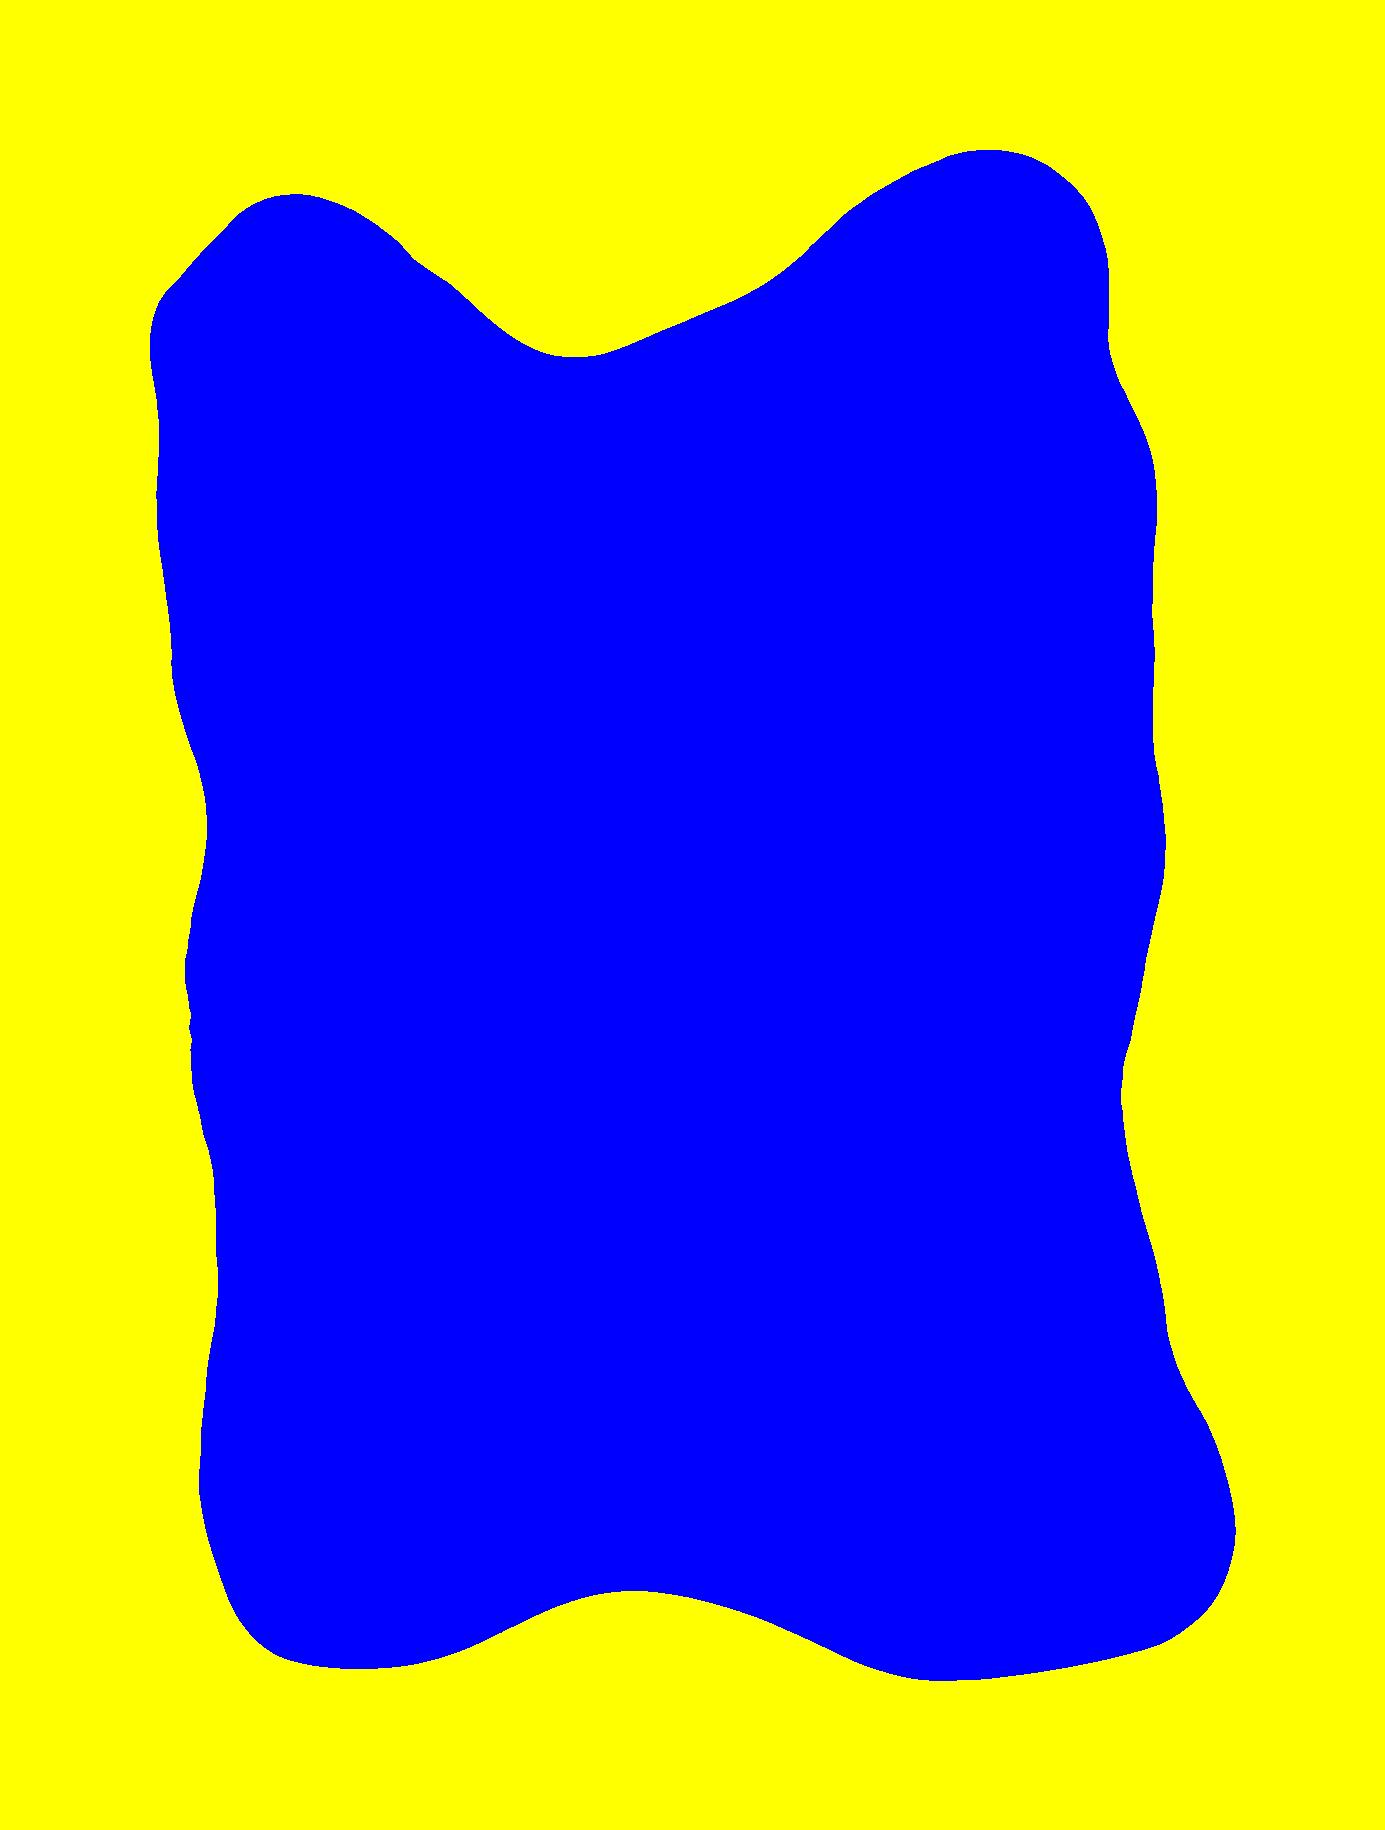
\includegraphics[width=.9\linewidth]{img/segmentation/good/watershed/segmented.jpg}
		\subcaption*{}
	\end{subfigure}
	\begin{subfigure}[b]{0.24\textwidth}
		\centering
		\includegraphics[width=.9\linewidth]{img/segmentation/bad/watershed/cut.jpg}
		\subcaption*{}
	\end{subfigure}
	\begin{subfigure}[b]{0.24\textwidth}
		\centering
		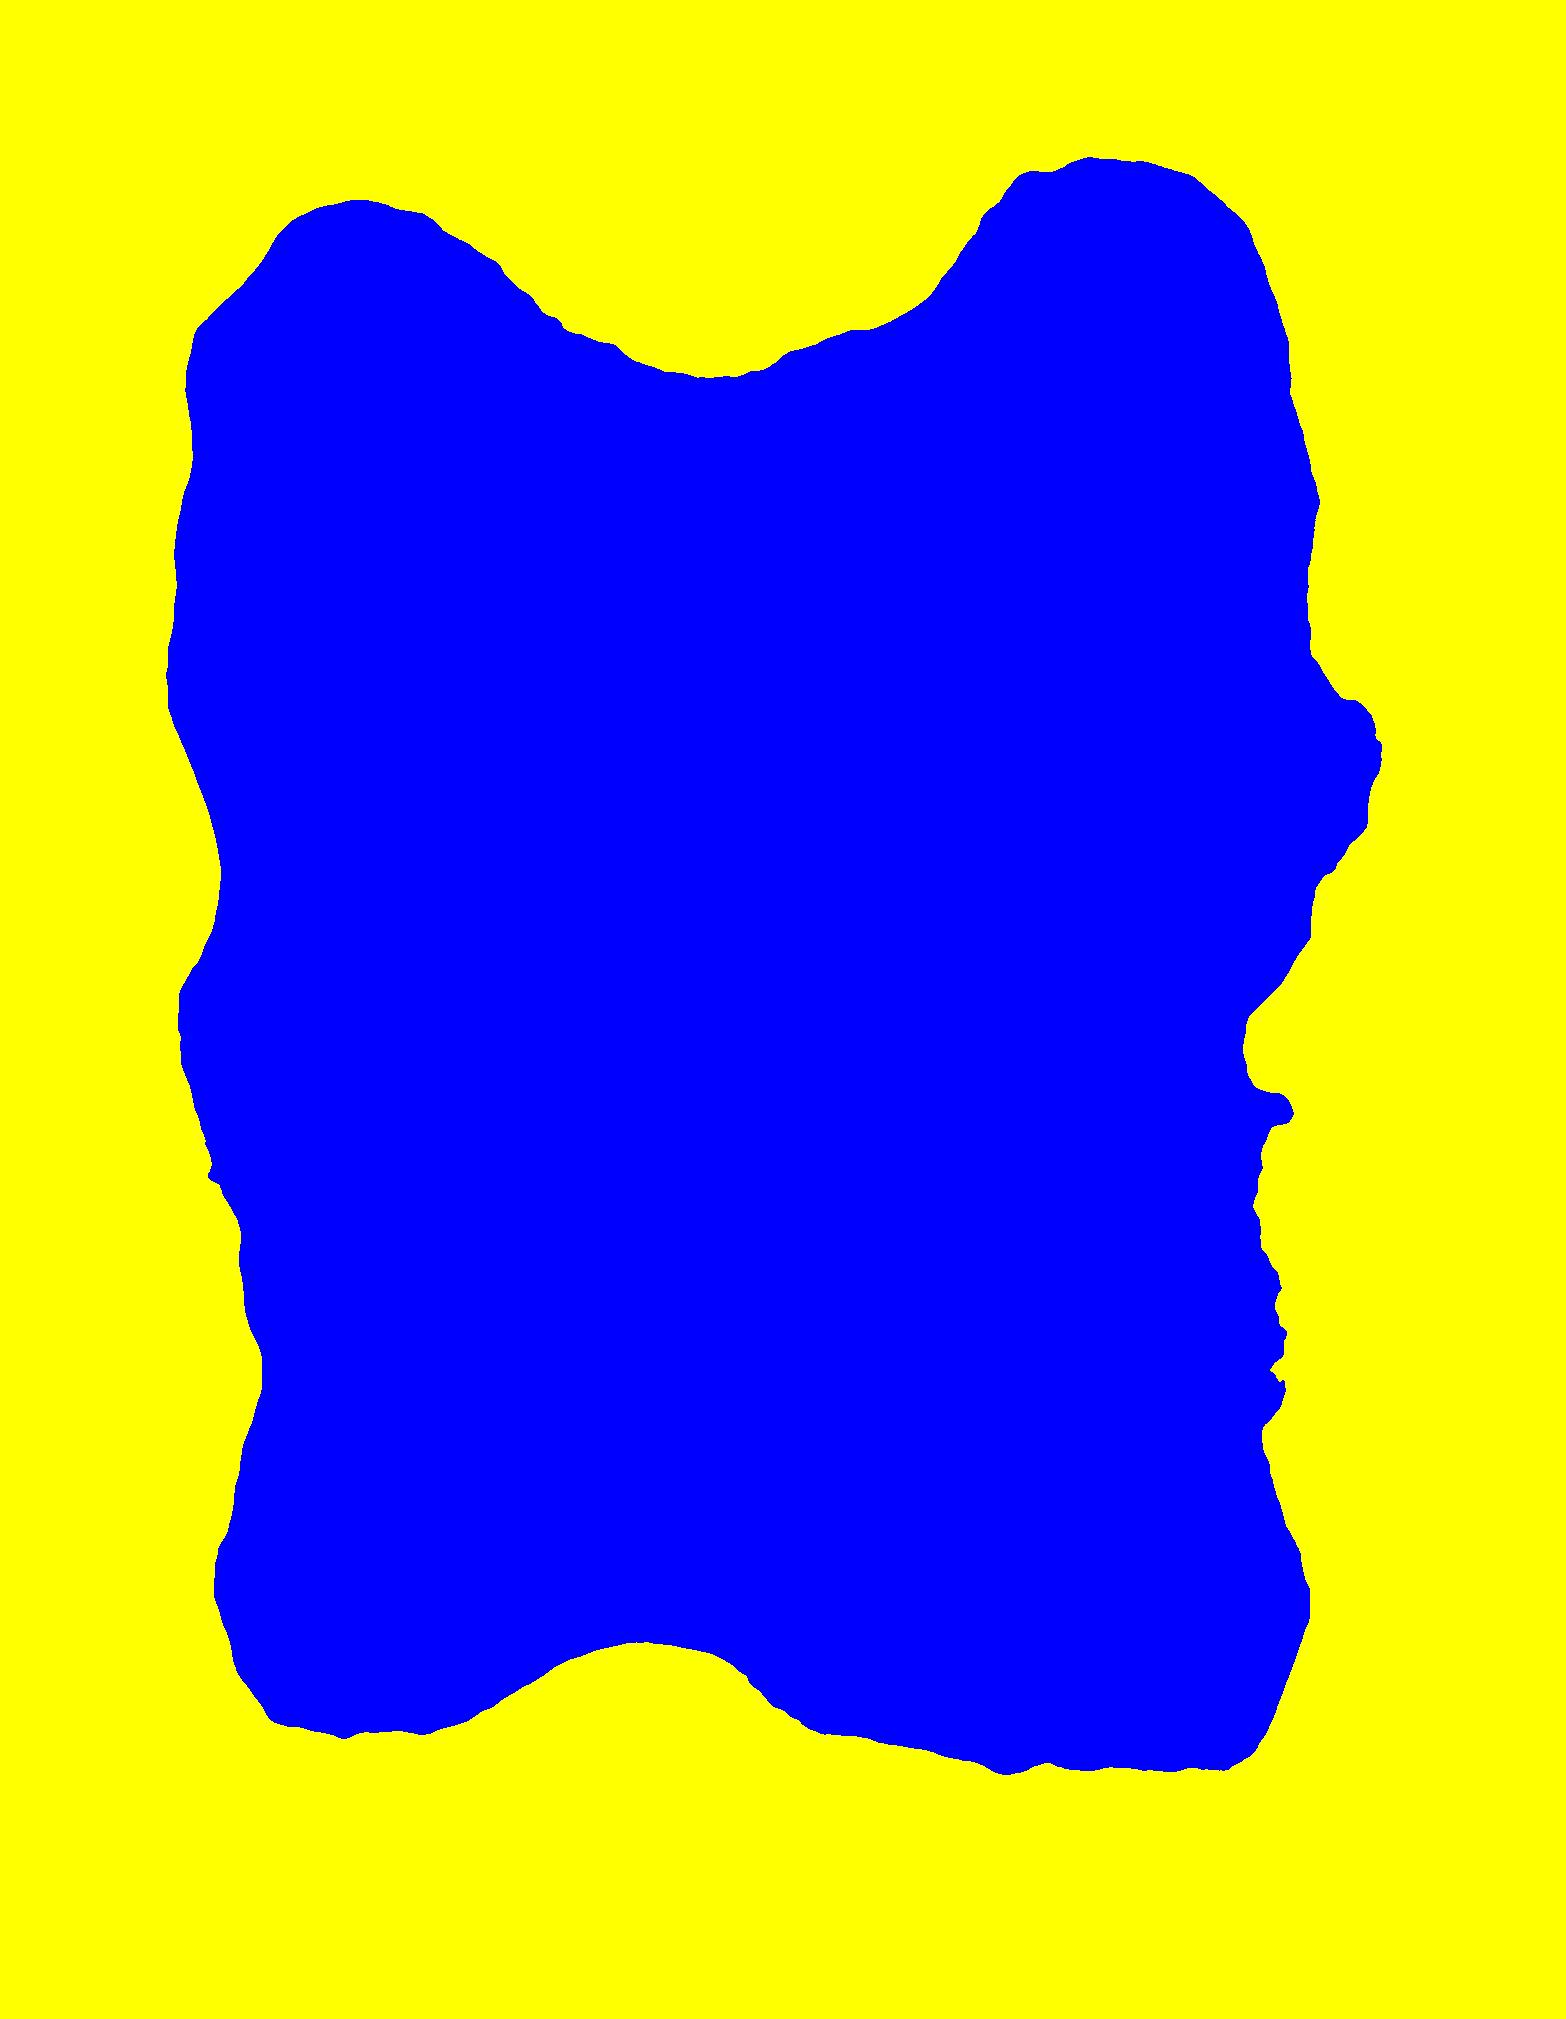
\includegraphics[width=.9\linewidth]{img/segmentation/bad/watershed/segmented.jpg}
		\subcaption{}
	\end{subfigure}
	\caption{Image Segmentation using watershed algorithm for two images}
	\label{fig:watershed}
\end{figure}

We chose the parameter $\mu$ as $1.25$ and used the largest resulting label as on-bone-pixels. While this yielded results that were sufficient to determine where the  location of the bone in the image is, the exact outline of the bone could not be reproduced using this method as visible in Figure \ref{fig:watershed}. Nevertheless we leveraged this method to limit the search space for the following segmentation methods by cutting out the bounding box of the bone from the rest of the image.

\subsubsection{SLIC}

Simple linear iterative clustering (SLIC) is a method proposed by Achanta et. al. in \cite{achanta2012slic} to extract areas of perceptual similarity from an image. While this is not a texture based method, by clustering the image into small regions of the same size we hoped to adhere to the edges of the bone. SLIC employs k-means clustering representing each pixel by its color values in the CIELAB color space and its position in the image. The parameter $k$ is the number of desired superpixels. An additional parameter $m$ can be supplied to weigh spatial and color information in the distance function of the cluster algorithm. A small value for $m$ leads to less densely packed superpixels that adhere more tightly to boundaries.

\begin{figure}[h]
	\centering
	\begin{subfigure}[b]{0.24\textwidth}
		\centering
		\includegraphics[width=.9\linewidth]{img/segmentation/good/slic/cut.jpg}
		\subcaption{}
		\label{fig:slic:good}
	\end{subfigure}
	\begin{subfigure}[b]{0.24\textwidth}
		\centering
		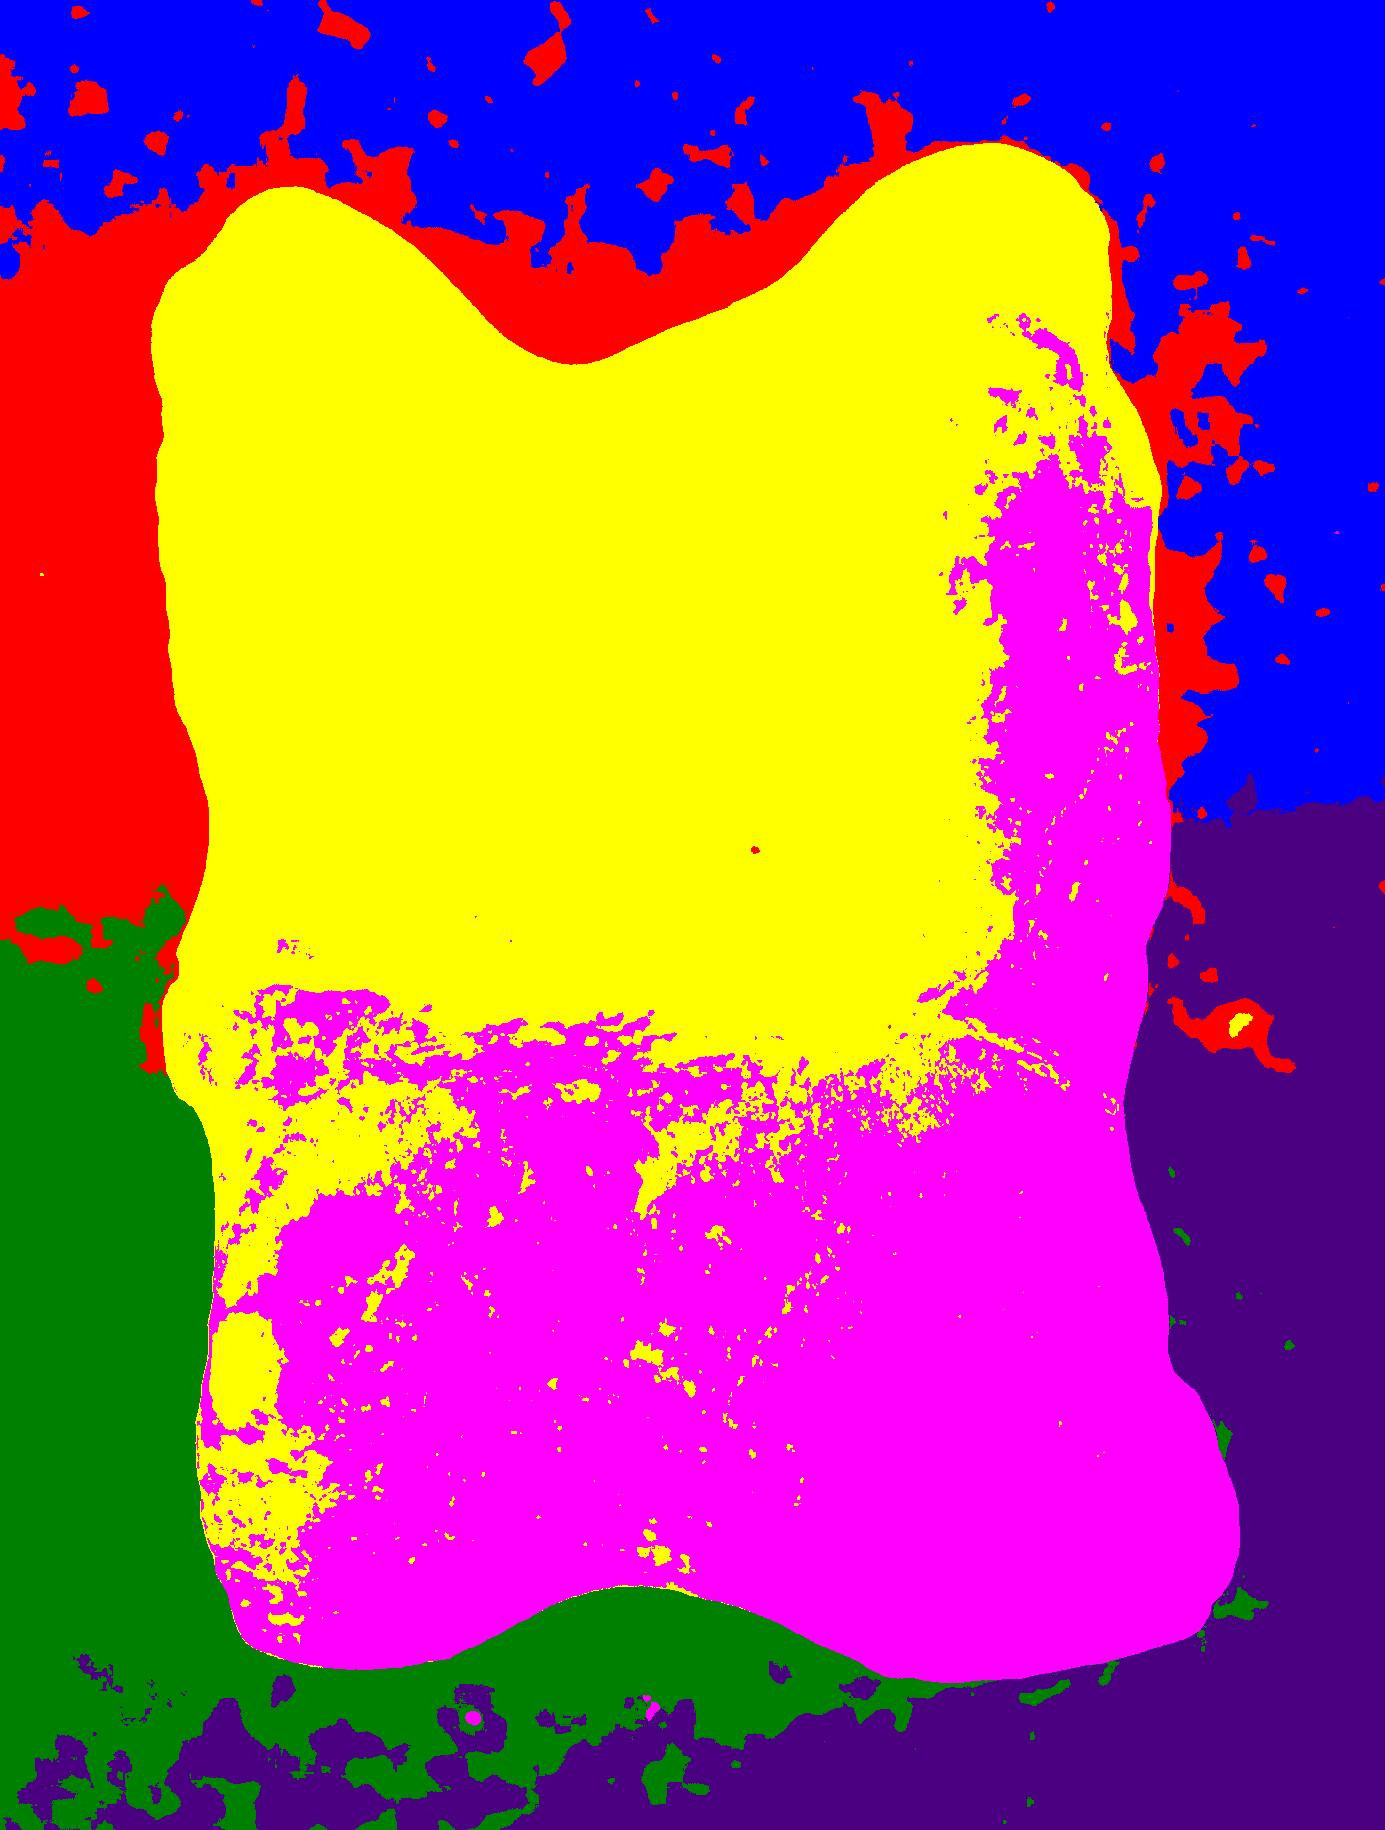
\includegraphics[width=.9\linewidth]{img/segmentation/good/slic/segmented.jpg}
		\subcaption*{}
		\label{}
	\end{subfigure}
	\begin{subfigure}[b]{0.24\textwidth}
		\centering
		\includegraphics[width=.9\linewidth]{img/segmentation/bad/slic/cut.jpg}
		\subcaption{}
		\label{fig:slic:bad}
	\end{subfigure}
	\begin{subfigure}[b]{0.24\textwidth}
		\centering
		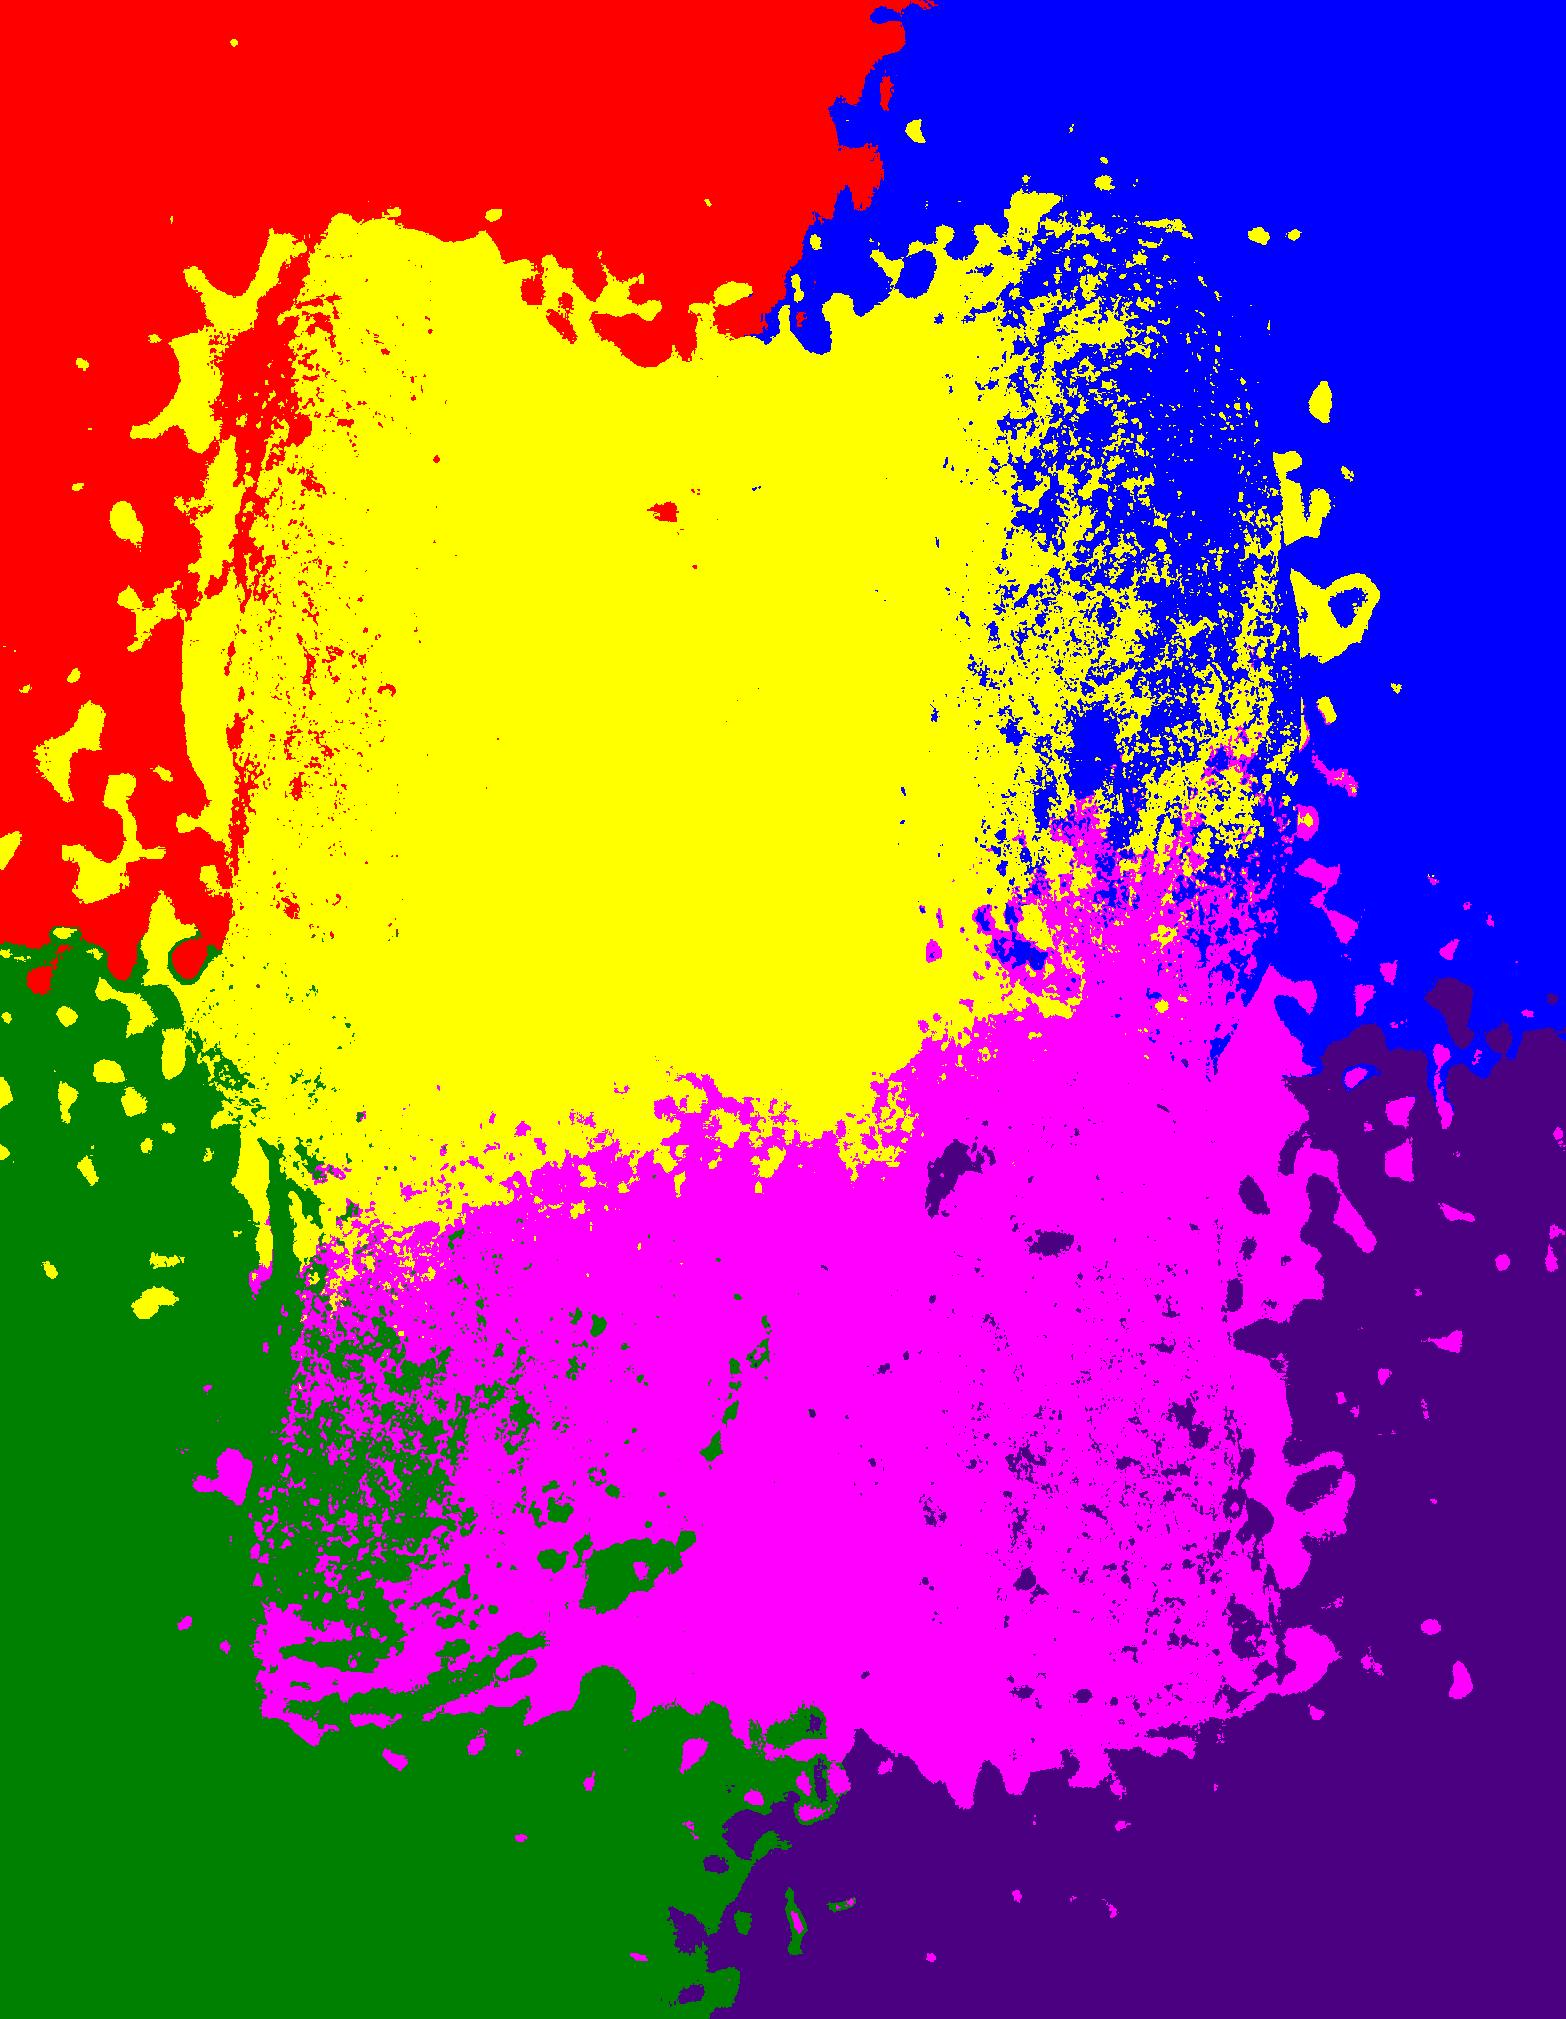
\includegraphics[width=.9\linewidth]{img/segmentation/bad/slic/segmented.jpg}
		\subcaption*{}
		\label{}
	\end{subfigure}
	\caption{Image Segmentation using SLIC superpixels for two images}
	\label{fig:slic}
\end{figure}

This superpixel method works well for images with differing background and foreground colors as visible in Figure \ref{fig:slic:good} and when using a sufficiently number of superpixels $k=8$. Increasing the weight $m$ to $m=15$ leads to compact clusters that align to the bone shape. When background and foreground colors are similar as it is the case in Figure \ref{fig:slic:bad}, the clusters become more frayed and do not align anymore with the bone shape.

\subsubsection{Felzenszwalb Graph-Based}

The method proposed by Felzenszwalb et. al in \cite{felzenszwalb2004efficient} is a graph based image segmentation method that works with the local neighborhoods of pixels. We decided to implement this method because it tries to segment perceptually similar regions. It works on the neighborhood graph of the image and defines the edges weights as the difference between the intensity of the pixels. The algorithm then iteratively splits and merges segments of the graph until the overall segmentation obeys certain global properties. The global properties are that the segmentation is neither too fine nor too coarse.

\begin{itemize}
	\item A segmentation $S$ is too fine if there is some pair of regions $C_1, C_2 \in S$ for which there is no evidence of a boundary between them
	\item A segmentation $S$ is too coarse when there exists a proper refinement of $S$ that is not too fine
\end{itemize}

The split algorithm can be configured by a parameter $k$, which sets the scale of observation. A larger $k$ means that stronger evidence for a boundary is needed to perform a split.

\begin{figure}[h]
	\centering
	\begin{subfigure}[b]{0.24\textwidth}
		\centering
		\includegraphics[width=.9\linewidth]{img/segmentation/good/felzenszwalb/cut.jpg}
		\subcaption{}
		\label{fig:felzenszwalb:good}
	\end{subfigure}
	\begin{subfigure}[b]{0.24\textwidth}
		\centering
		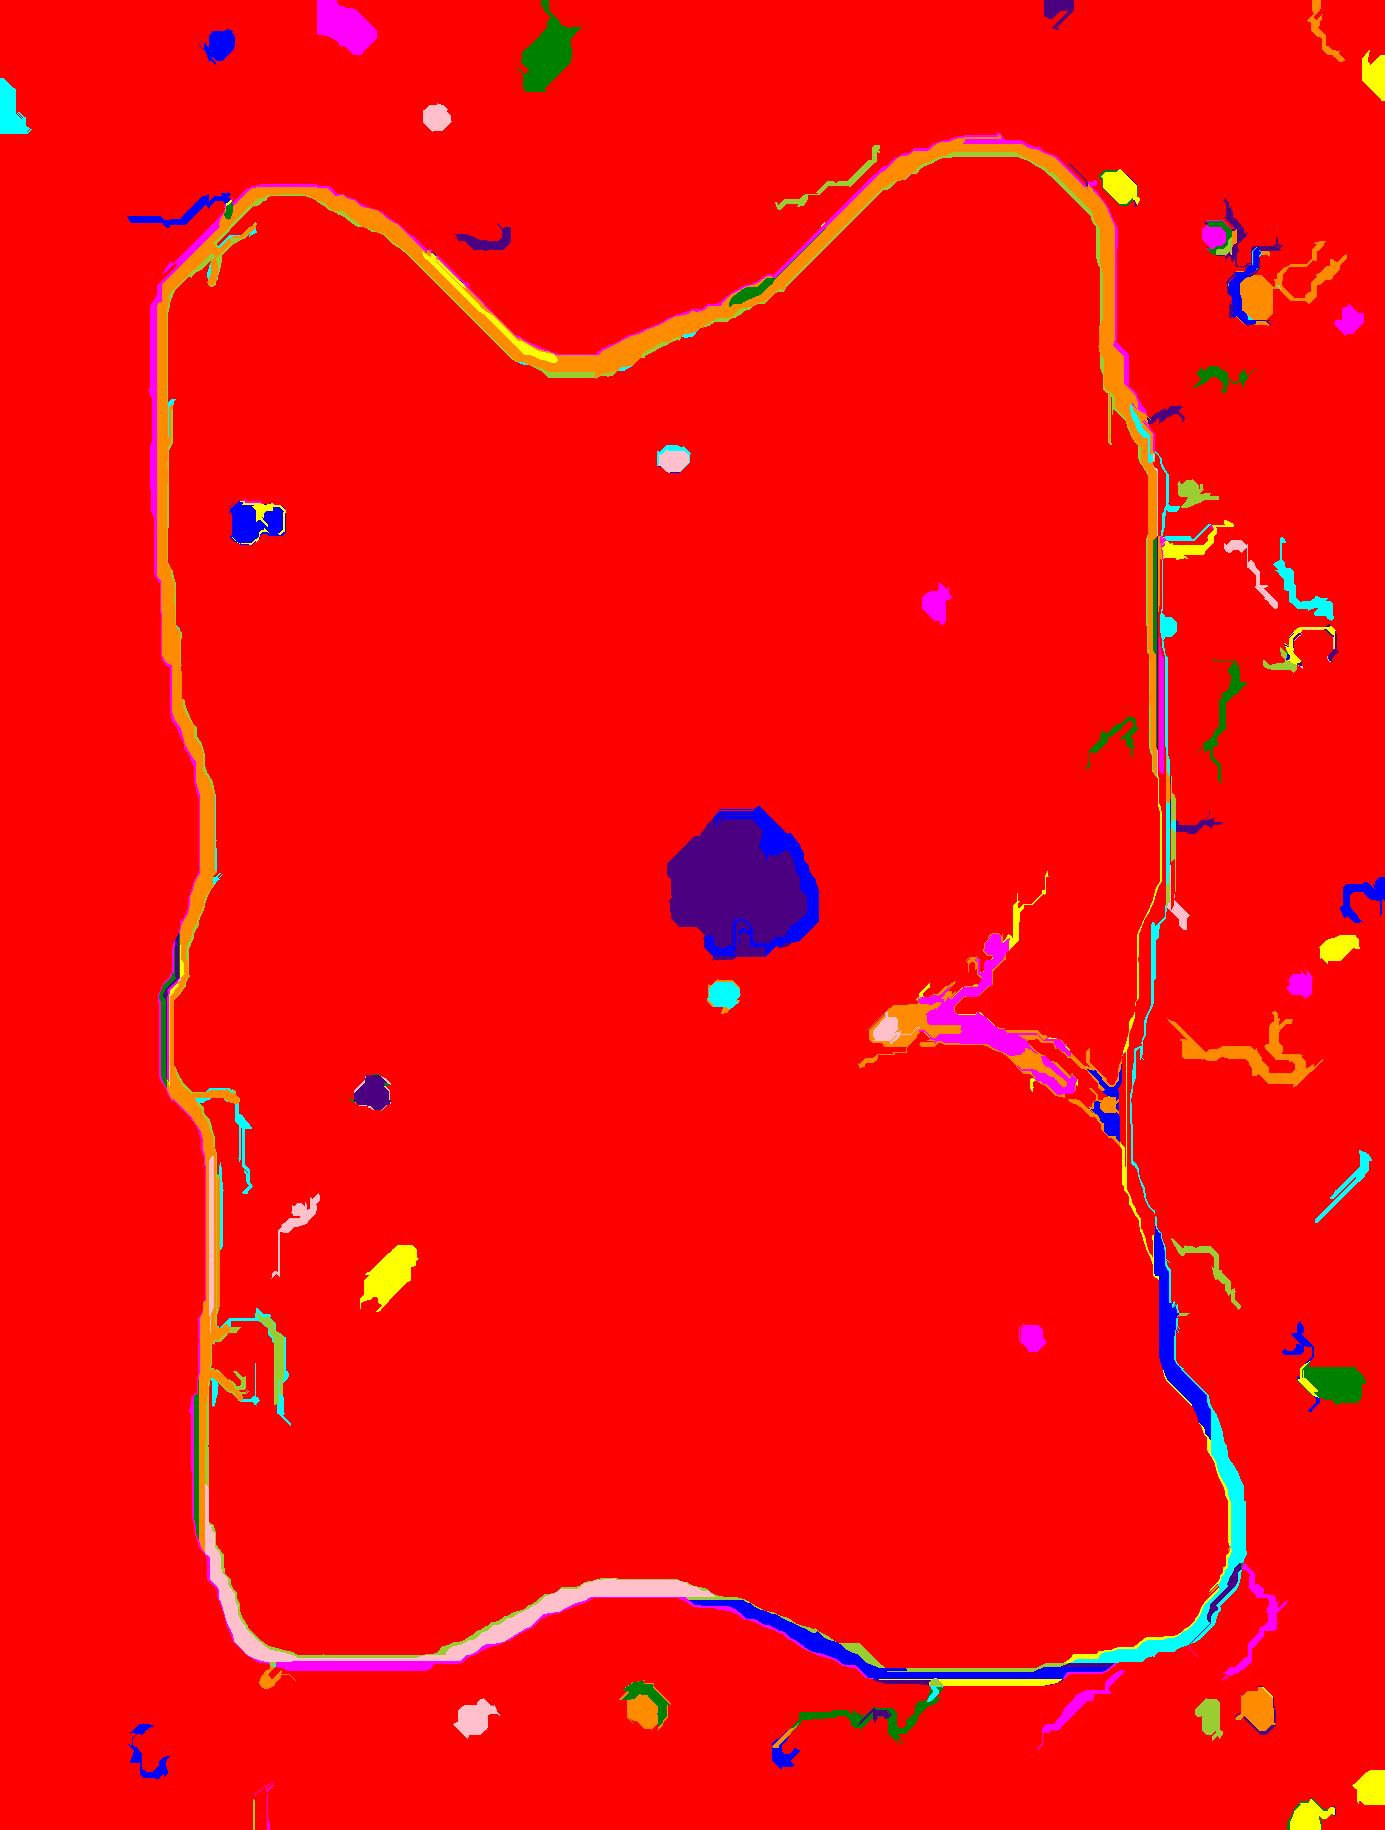
\includegraphics[width=.9\linewidth]{img/segmentation/good/felzenszwalb/segmented.jpg}
		\subcaption*{}
		\label{}
	\end{subfigure}
	\begin{subfigure}[b]{0.24\textwidth}
		\centering
		\includegraphics[width=.9\linewidth]{img/segmentation/bad/felzenszwalb/cut.jpg}
		\subcaption{}
		\label{fig:felzenszwalb:bad}
	\end{subfigure}
	\begin{subfigure}[b]{0.24\textwidth}
		\centering
		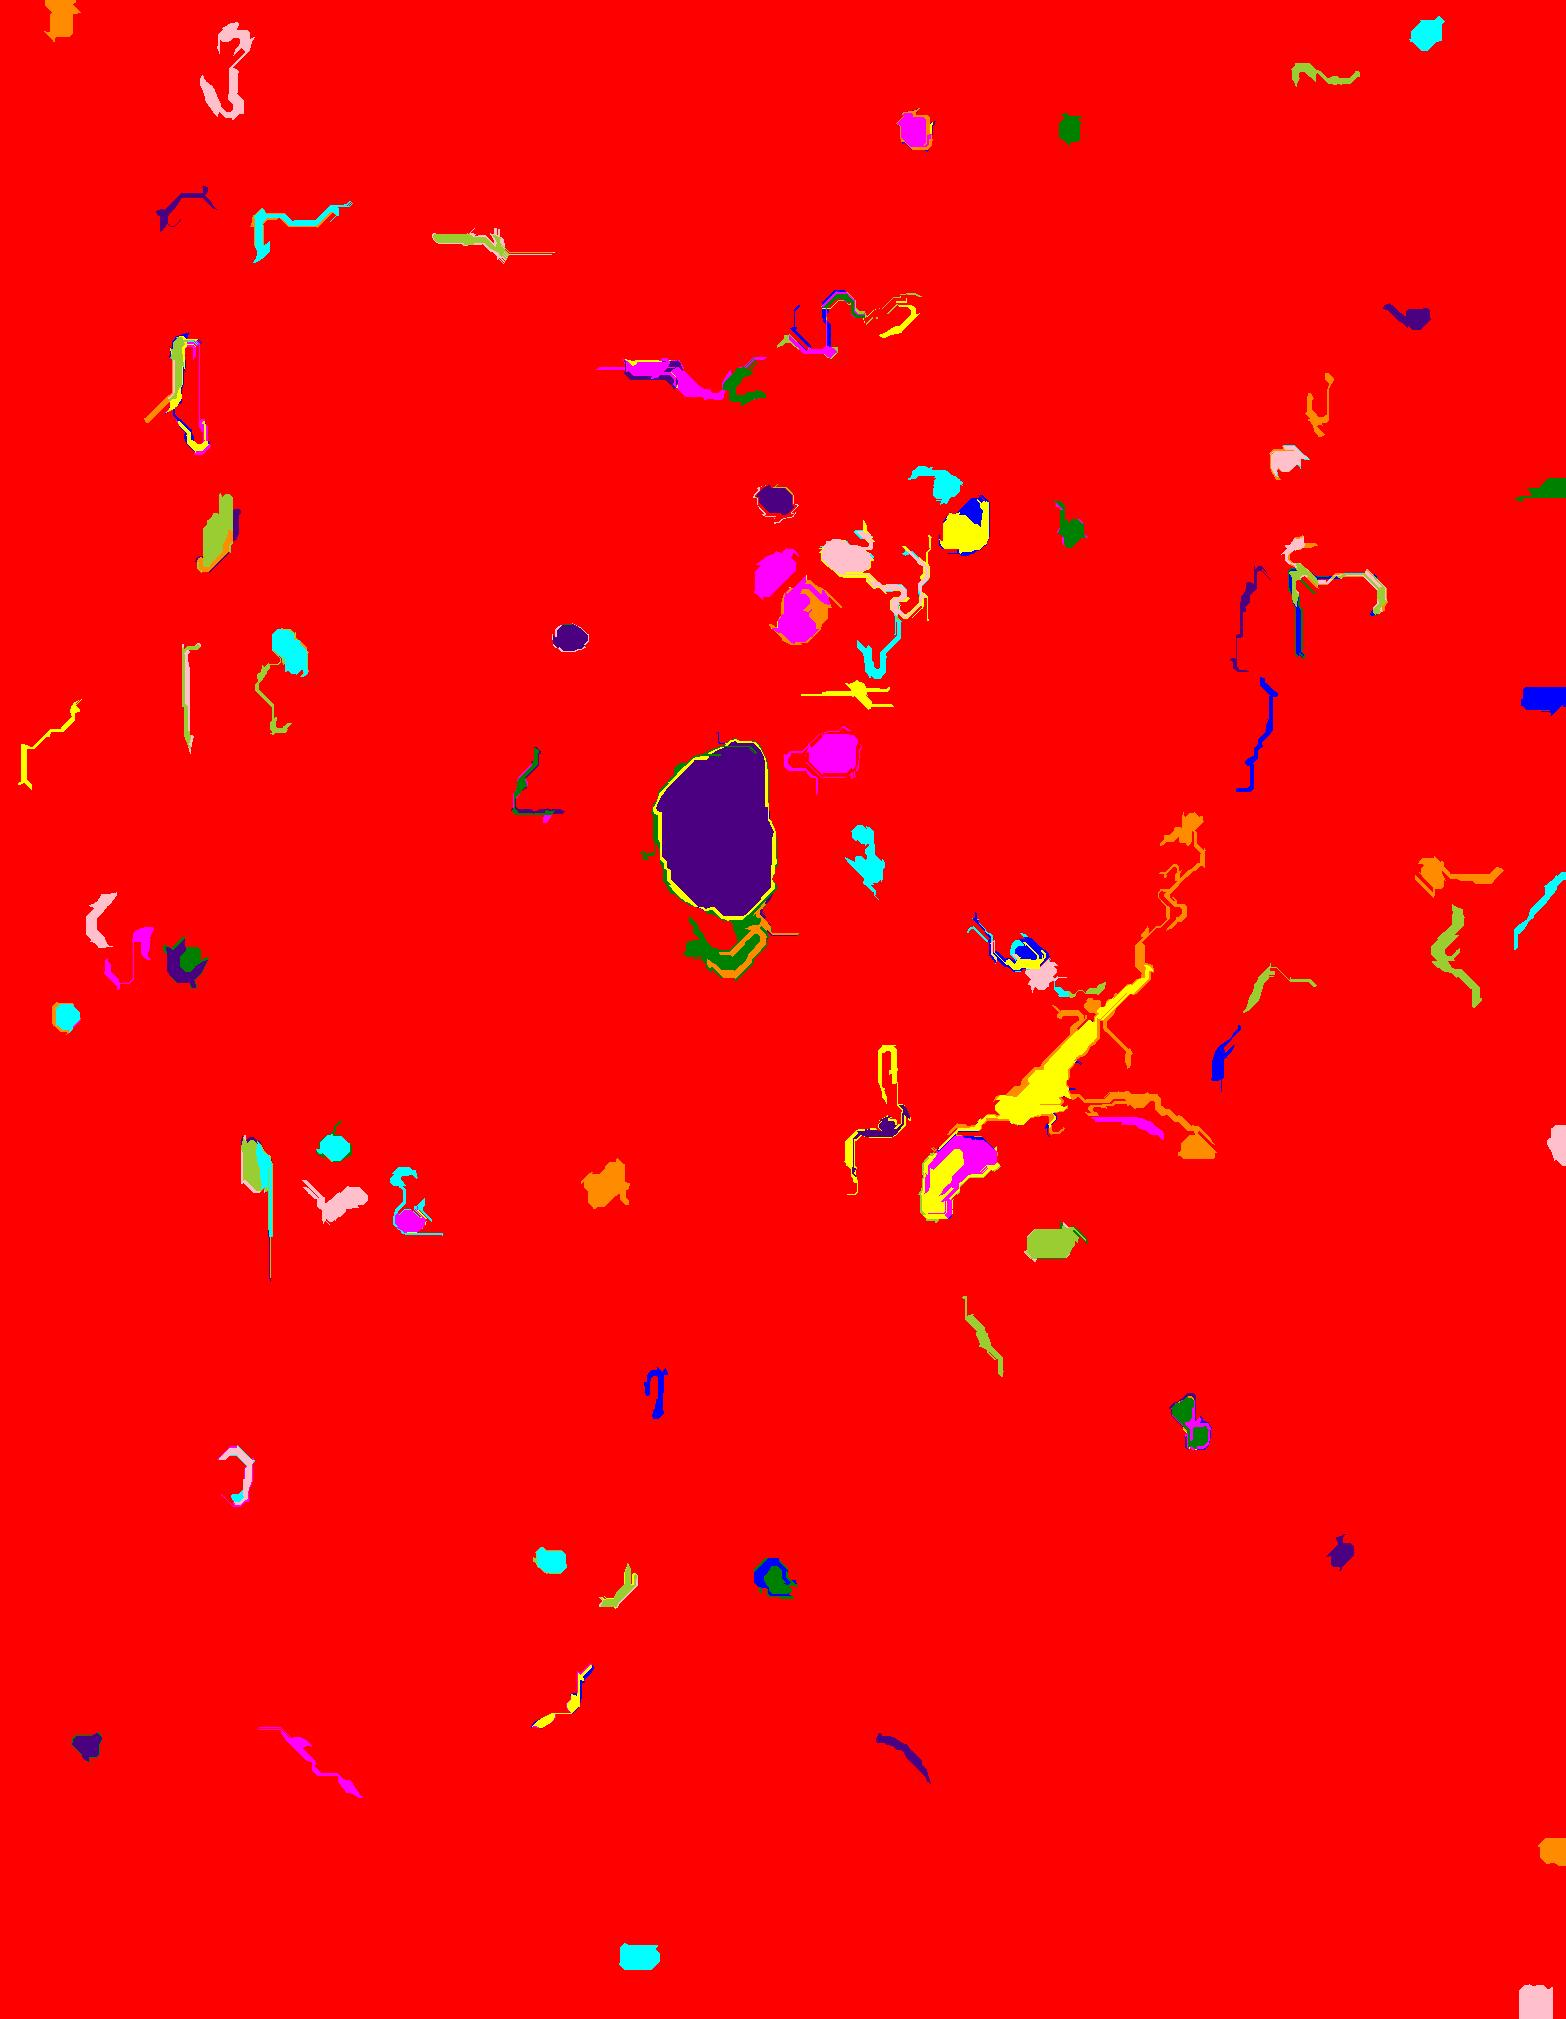
\includegraphics[width=.9\linewidth]{img/segmentation/bad/felzenszwalb/segmented.jpg}
		\subcaption*{}
		\label{}
	\end{subfigure}
	\caption{Image Segmentation using Felzenszwalb's graph-based method for two images}
	\label{fig:felzenszwalb}
\end{figure}

In contrast to the previous methods, Felzenszwalb's method creates clusters from the edge of the bone only as shown in Figure \ref{fig:felzenszwalb:good}. These labels adhere to the edges of the bone, but some additional areas are included in the result as well. The number of labels is not selectable and for large images this method can create hundreds of labels, which complicates label selection for the user, so a sufficiently high observation level $k$ needs to be chosen to reduce the number of labels. For our purpose, we chose $k=1000$. The images that are difficult to segment could often not be correctly segmented using this method as visible in Figure \ref{fig:felzenszwalb:bad}. When choosing a small value for $k$ a huge amount of small labels was generated. On the other hand, when choosing a large value for $k$, the bone and background collapsed into a single label.

\subsubsection{Semi-local region descriptor}

The method based on a semi-local region descriptor and active contour by Houhou et. al. in \cite{houhou2009fast} is the first method presented here that relies on a description of the texture that surrounds a pixel. The texture feature $F$ presented in the paper analyzes a patch $P_{x,y}$ around the pixel at position $(x,y)$ and represents the texture of this patch by a manifold. The metric
tensor of this method is then calculated, accumulated for all color channels and a textural feature is extracted from the metric tensor.

For the sake of simplicity we decided only to implement the texture feature from \cite{houhou2009fast} and not the proposed segmentation method, since the documentation was very sparse.

TODO: Results

\subsubsection{Gabor Filters}

Another way to do texture segmentation in images is to represent the image using Gabor filters. The image is decomposed using Gabor filters into a number of filtered images that each contain variations in intensity over a certain frequency and in a certain direction. To obtain filtered images for segmentation it is necessary to well define the parameters of the filters. We used the filter selection method from \cite{jain1990unsupervised} to obtain the filter parameters. Gabor filters are tailored to represent the early stages of the human visual system, so the image is preprocessed using a non-linear function first and then the filters with the selected parameters are applied. This results in an vector of pixel values per pixel that can be clustered using k-means.

\begin{figure}[h]
	\centering
	\begin{subfigure}[b]{0.24\textwidth}
		\centering
		\includegraphics[width=.9\linewidth]{img/segmentation/good/gabor/cut.jpg}
		\subcaption{}
		\label{fig:gabor:good}
	\end{subfigure}
	\begin{subfigure}[b]{0.24\textwidth}
		\centering
		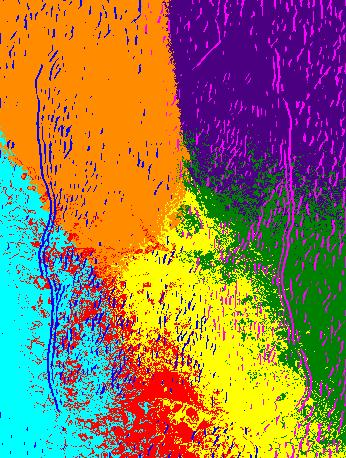
\includegraphics[width=.9\linewidth]{img/segmentation/good/gabor/segmented.jpg}
		\subcaption*{}
		\label{}
	\end{subfigure}
	\begin{subfigure}[b]{0.24\textwidth}
		\centering
		\includegraphics[width=.9\linewidth]{img/segmentation/bad/gabor/cut.jpg}
		\subcaption{}
		\label{fig:gabor:bad}
	\end{subfigure}
	\begin{subfigure}[b]{0.24\textwidth}
		\centering
		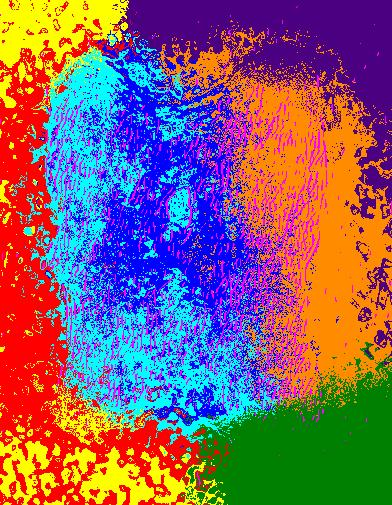
\includegraphics[width=.9\linewidth]{img/segmentation/bad/gabor/segmented.jpg}
		\subcaption*{}
		\label{}
	\end{subfigure}
	\caption{Image Segmentation using Gabor filters for two images}
	\label{fig:gabor}
\end{figure}

The results of clustering the Gabor filter features vary heavily depending on the image. For almost all images, wavy features either in the background or on the bone are detected. Depending on where they are detected, one of these labels can be used to outline the bone. As visible in Figure \ref{fig:gabor} this sometimes works better for difficultly separable images.

\subsubsection{Textural Edge Detection}

An approach to edge detection using semi-local texture features was also implemented. Since it wasn't necessary to segment the whole bone as on-bone-pixels but only the outline, we defined the outline as a region where there are different textures on either side. To detect vertical and horizontal edges we considered the local neighborhood of $n$ pixels into each direction of the pixel $N_{left}(x,y), N_{right}(x,y), N_{top}(x,y), N_{bottom}(x,y)$.

\begin{equation}
\begin{split}
	& N_{left}(x,y) = \{ (x-n,y), (x-1,y) \} \\
	& N_{right}(x,y) = \{ (x+1,y), (x+n,y) \} \\
	& N_{top}(x,y) = \{ (x,y+n), (x,y+1) \} \\
	& N_{bottom}(x,y) = \{ (x,y-1), (x,y-n) \}
\end{split}
\end{equation}

We then calculated textural features $F$ for these local neighborhoods and used the distance between them as a measure for an edge. For this purpose we used Haralick textural features (\cite{haralick1973textural}) or parameter free threshold adjacency statistics (\cite{hamilton2007fast}). 

\begin{equation}
\begin{split}
E(x,y) = & ||F(N_{left}(x,y)) -F(N_{right}(x,y))|| \\ & + ||F(N_{top}(x,y)) - F(N_{bottom}(x,y))||
\end{split}
\end{equation}

\begin{figure}[h]
	\centering
	\begin{subfigure}[b]{0.24\textwidth}
		\centering
		\includegraphics[width=.9\linewidth]{img/segmentation/good/textural-edges/cut.jpg}
		\subcaption{}
		\label{fig:textural:good}
	\end{subfigure}
	\begin{subfigure}[b]{0.24\textwidth}
		\centering
		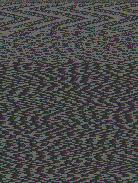
\includegraphics[width=.9\linewidth]{img/segmentation/good/textural-edges/segmented.jpg}
		\subcaption*{}
		\label{}
	\end{subfigure}
	\begin{subfigure}[b]{0.24\textwidth}
		\centering
		\includegraphics[width=.9\linewidth]{img/segmentation/bad/textural-edges/cut.jpg}
		\subcaption{}
		\label{fig:textural:bad}
	\end{subfigure}
	\begin{subfigure}[b]{0.24\textwidth}
		\centering
		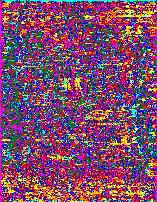
\includegraphics[width=.9\linewidth]{img/segmentation/bad/textural-edges/segmented.jpg}
		\subcaption*{}
		\label{}
	\end{subfigure}
	\caption{Image Segmentation using textural edge detection for two images}
	\label{fig:textural}
\end{figure}

The results for this segmentation method are mixed as well. While edges are detected correctly on images with high contrast as visible in Figure \ref{fig:textural:good}, the results appear random for images with low contrast between bone and background as shown in Figure \ref{fig:textural:bad}. Some structure is visible in Figure \ref{fig:textural:bad}, but the clustering does not work well in this case because of the low number of features.

\subsection{Triangulation and Outlining}

The next step for preprocessing images was extracting the outline from a segmented image. As stated in Section
\ref{sub:segmentation}, we marked some pixels in the images as being pixels that lie on the bone.
To extract the outline from these pixels, we first transformed them into points in the x-y-space and then
triangulated them using the Delaunay triangulation.

To reduce the number of outliers that were detected as on-bone-pixels,
we decided to use the DBSCAN algorithm from \cite{ester1996density} and apply density based clustering to the points
beforehand. DBSCAN allowed us to create clusters from the data, which correspond to closely packed points. Since
the points on the bone were closely packed, and the points not on the bone were only sparsely detected as
on-bone-pixels this allowed us to filter some of the false-positives. Another benefit of the DBSCAN algorithm is that,
by defining our bone as a large densely connected area, we were able to use the largest cluster from the result,
so closely packed areas that are disconnected from the bone were also removed.

The Delaunay triangulation was applied to the remaining points to create a triangulated mesh. Since Delaunay
triangulation can only create meshes with convex outlines, another step was required to extract the bone outline
from the triangulation. For this purpose we used the $\alpha$-complex of the mesh as defined in \cite{akkirajualpha}.
The $\alpha$-complex algorithm removes outer triangles for the Delaunay triangulation that have a radius which exceeds
$\frac{1}{\alpha}$. $\alpha$ is a parameter and was chosen as $25$ for our purpose, which provided us with
an accurate concave outline of the bone.

Since we are analyzing the shape of the object, a manual step was introduced here to give the user the ability to
approve the automatically extracted outline and adapt it if the result was not satisfactory. We gave the user the
ability to mark points as on-the-bone/off-the-bone as well as fill a rectangle with a grid of on-the-bone points (or mark them all as not on-the-bone).
This allows the user to easily adapt a triangulation and, if necessary, create a completely new one. It becomes
especially important because the result of the image segmentation algorithm often has jagged borders, because the
image segmentation algorithms do not consider the smoothness of the outline.

Since the bones might have different sizes and positions, due to different image sizes and position of the bone in
the image, we needed to introduce another normalization step afterwards. We decided to remove all variance in between the bones that are not attributed to shape. For this purpose we executed the first two steps of Procrustes
analysis, also used in Section \ref{subsub:procrustes}.

\begin{itemize}
	\item Transformation of all point sets into the coordinate center
	\begin{equation}
		\begin{split}
			& \bar{x} = \frac{x_{1x} + x_{2x} + \cdots + x_{nx}}{n} \\
			& \bar{y} = \frac{x_{1y} + x_{2y} + \cdots + x_{ny}}{n} \\
			& X_c = \{ (x_{1x} - \bar{x}, x_{1y} - \bar{y}), \cdots, + (x_{nx} - \bar{x}, x_{ny} - \bar{y}) \}
		\end{split} 
	\end{equation}
	\item Scaling all point sets uniformly
	\begin{equation}
		\begin{split}
			& s = \sqrt{\frac{\sum\limits_{x \in X_c}||x||^2}{n}} \\
			& X_s = \left\{ \frac{x_{c1}}{s}, \cdots, \frac{x_{cn}}{s}\right\}
		\end{split}
	\end{equation}
\end{itemize}

\subsection{Landmark Extraction}
\label{sub:landmarks}

As some of the features we propose in this work are landmark based, and the detection of on-site-measurable differences
is based on landmarks as well, a method to extract these landmarks from the outline of the bone is needed. In contrast to
our approach, former work on the talus by zooarcheologists was based on manually located landmarks that correspond to
biological features of the bone. Since our goal was to automate the process as much as possible and some of the landmarks
are not positioned on the outline of the bone, this was not feasible in our case. We selected landmarks on the outline
of the bone that could be located automatically and overlap as much as possible with the landmark definitions by the
zooarcheologists. For this purpose we introduced two methods that extract landmarks from outlines of Tali. The landmarks
found by these methods have very similar positions but differ in on-site-measurability and stability in-between classes.

Figure \ref{figure-landmark-methods} shows the results of the three landmark locating methods: manual, with angles and
with space partitioning. The biological correspondences of the landmarks are as follows.

\begin{itemize}
\item Landmark 1: Highest point on the lateral crest
\item Landmark 2: Lowest point in between the crests
\item Landmark 3: Highest point on the medial crest
\item Landmark 4: Intersection between the medial outer edge and the medially arcing edge of the medial crest
\item Landmark 5: Out most point on the medial apex
\item Landmark 6: Lowest point on the medial outer edge
\item Landmark 7: Highest point on the distal depression
\item Landmark 9: Intersection of the distal articular surface with the Calcaneus
\item Landmark 10: Lateral end point of the lower muscle attachment line
\item Landmark 11: Intersection of the two muscle attachment lines
\item Landmark 12: Proximal end point of the lateral protrusion on the lateral crest
\end{itemize}

The landmarks that were extracted automatically are landmarks 1, 2, 3, 5, 6, 7. Furthermore we introduced the new
landmark 8, which has no biological correspondence, but can be located robustly on all bone outlines.

\subsubsection{Extraction by Angle}

When extracting a landmark by angle, the landmark position is defined by a minimum angle $\alpha_{min}$, a maximum
angle $\alpha_{max}$ and the information whether it is located on a minimum or a maximum turning point.
The minimum/maximum turning angle $\alpha_{t}$ between $\alpha_{min}$ and $\alpha_{max}$ of the following function
is calculated, where $i(\alpha)$ is the intersection between a ray from the coordinate center with the angle $\alpha$ and
the outline. $i(\alpha_t)$ is then used as the landmark.

\begin{equation}
d(\alpha) = ||i(\alpha)||
\end{equation}

The definitions for all landmarks when using this method can be found in Appendix \ref{appendix:table:landmarks-angle}.

The landmarks found by this method are robustly located across all classes, but have a distinct disadvantage. They are
not as easily located by hand since they dont lie exactly on the high points of the outline, but slightly beneath
them  as seen in Figure \ref{figure-landmark-methods}. This makes distances in between landmarks harder to measure, which
will become relevant in Chapter \ref{chapter:measurable-differences}.

\subsubsection{Extraction by Space Partitioning}

When extracting a landmark by space partitioning, the landmark position is defined by a rectangle in which the landmark
lies, the information whether it lies on a maximum or a minimum turning point and the coordinate axis on which the
turning point lies. The rectangle is defined by $x_{min}$, $x_{max}$, $y_min$ and $y_max$. The turning point
is then found by only evaluating the respective axis inside the rectangle. The following function for turning points
is then evaluated inside the rectangle, where $s_y(x)$ is the x-coordinate of the spline at the x-coordinate $x$.

\begin{equation}
d(x) = s_y(x)
\end{equation}

The definitions for all landmarks when using the space-partitioning method can be found in Appendix
\ref{appendix:table:landmarks-space}.

When looking at the landmarks found by this method, they tend to lie exactly on the high points of the outline, which
makes them easily locatable by hand. The drawback of this approach is that local high or low points can be mistaken as
landmarks by this algorithm, especially when the bone shapes are not registered yet.

\section{Shape Registration}

To adequately compare the shapes, we needed to align them first as much as possible, so small differences in shape would
show in the result. For this purpose we implemented several methods for point-to-point registration algorithms in order
to find the one that best matches our dataset. In general point-to-point registration algorithms that matches point set
$X$ onto point set $Y$ consist of two parts:

\begin{itemize}
\item Find correspondent points $C_Y$ for (some of the) points in $X$
\item Find transformation $T$ that aligns $X$ to $C_Y$ as best as possible under certain restrictions
\end{itemize}

We chose the reference point set $Y$ to be represented by the bone outline with the most points, since this will allow
us to find non-duplicate correspondences from $X$ to $Y$. Since we are considering the outline of the bone and not
individual points, we can choose any points on the outline $B_Y$ as $Y$ and any point on the outline $B_X$ as $X$.
Transformation estimations can also easily be iterated as done by the ``Iterative Closest Point`` method \cite{besl1992method}.
The method can be different in each iteration. We implemented several methods for point-to-point correspondence
approaches as well as several for the estimation of the transformation which have different restrictions.

\begin{figure}[h]
	\centering
	\begin{subfigure}[b]{0.34\textwidth}
		\centering
		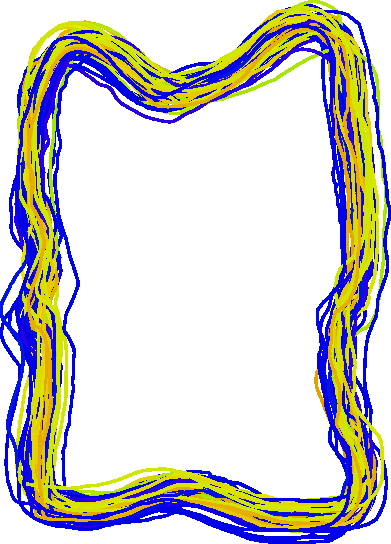
\includegraphics[width=.9\linewidth]{img/registration/unregistered.pdf}
	\end{subfigure}
	\hspace{0.1\textwidth}%
	\begin{subfigure}[b]{0.34\textwidth}
		\centering
		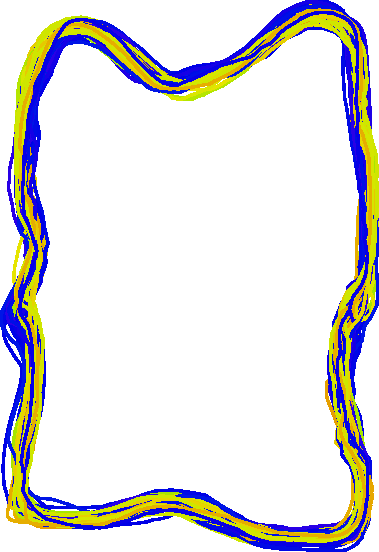
\includegraphics[width=.9\linewidth]{img/registration/registered.pdf}
	\end{subfigure}
	\caption{The bone outlines before (left) and after registration (right)}
	\label{fig:registration}
\end{figure}

Figure \ref{fig:registration} shows the bone outlines before and after the registration step. The differences between the two classes of bones, displayed as yellow and blue here, become more apparent.

\subsection{Correspondence Estimation}

Corresponding points are defined as pairs of semantically identical points in both point sets. Based on these
pairs, the transformation estimation is done.

\subsubsection{Landmarks}

When estimating the correspondence using landmarks, the landmark points are located as described in Section
\ref{sub:landmarks}. Since the number of landmarks is always the same in both outlines, we used the result
as one-to-one correspondences for the registration. We implemented both the angle-based as well as the
space-partitioning-based approaches of the automated landmark extraction. Additionally, we added a method
that evaluates the manually set landmarks of the bones.

\subsubsection{Spline Points}

Another approach to find correspondences was to parameterize the bone outline using a spline and then using $n$
evaluated points on the spline as a normalized representation of the shape. The spline representation consists
of two functions $s_x$, $s_y$ for the $x$ and $y$ coordinates of the outline. We evaluated this spline using $n$
equally spaced parameters $T$ as seen in Equation \ref{eq:registration-spline}.

\begin{equation}
\label{eq:registration-spline}
\begin{split}
& s(t) = ( s_x(t), s_y(t) ) \text{ with } 0 \leq t \leq 1 \\
& T = \{ t_i=\frac{i}{n} | i=0, 1, \dots, (n-1) \} \\
& X = \{ s(t_i) | t_i \in T \}
\end{split}
\end{equation}

These spline points can be evaluated for all bones in the bone set and provide a one-to-one estimation of correspondences.

\subsubsection{Nearest Neighbors}

All previously suggested approaches have one distinct disadvantage: The correspondences are static, meaning they don't
change after an iteration (although the positions of the automatically found landmarks might change). To compensate this
we implemented a nearest-neighbor approach to estimate correspondences. The resulting algorithm is very similar to
\cite{besl1992method} but uses other transformation estimators.

To find the correspondences for $X$ in $Y$ we simply use the nearest neighbor $NN_Y(x_i)$ for each point $x_i$ in $X$.

\begin{equation}
NN_Y(x_i) = \arg\min(\{ \forall y_i \in Y: dist(x_i, y_i) \})
\end{equation}

The correspondences found with this method might change after each iteration. This is beneficial for already registered
outlines.

\subsection{Transformation Estimation}

The transformation estimation is done for the selected corresponding points only and then applied to all points in
the point set.

\begin{figure}[h]
	\centering
	\begin{subfigure}[b]{0.24\textwidth}
		\centering
		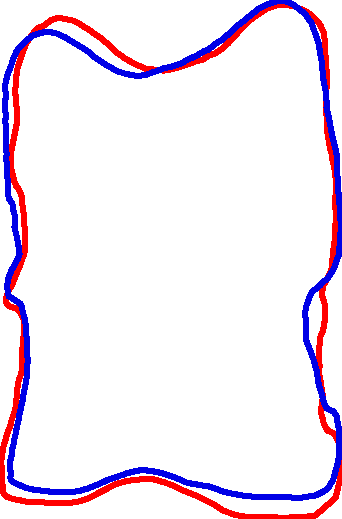
\includegraphics[width=.9\linewidth]{img/registration/single-before.pdf}
		\subcaption{unregistered}
	\end{subfigure}
	\begin{subfigure}[b]{0.24\textwidth}
		\centering
		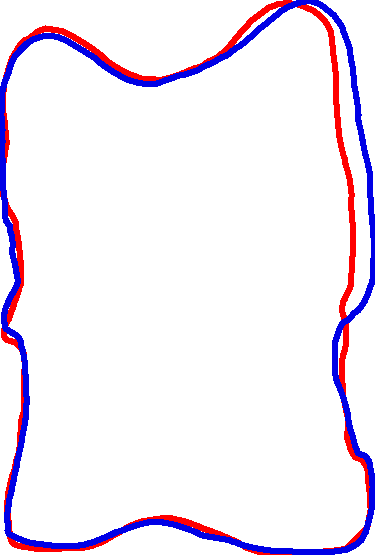
\includegraphics[width=.9\linewidth]{img/registration/single-procrustes.pdf}
		\subcaption{Procrustes}
	\end{subfigure}
	\begin{subfigure}[b]{0.24\textwidth}
		\centering
		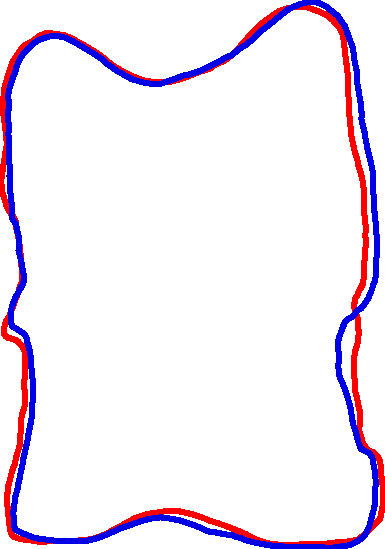
\includegraphics[width=.9\linewidth]{img/registration/single-affine.pdf}
		\subcaption{affine}
	\end{subfigure}
	\begin{subfigure}[b]{0.24\textwidth}
		\centering
		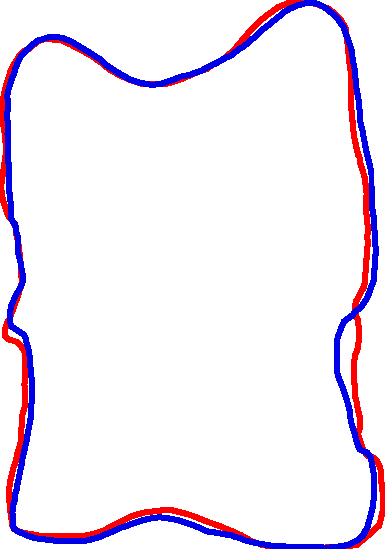
\includegraphics[width=.9\linewidth]{img/registration/single-projective.pdf}
		\subcaption{projective}
	\end{subfigure}
	\caption{A single registration step using same correspondences but different transformation estimations}
	\label{fig:slic}
\end{figure}

\subsubsection{Procrustes Transformation}
\label{subsub:procrustes}

Procrustes transformation is a transformation that uses a combination of translation, scaling and rotation. This kind of
transformation preserves the original shape of the object, making it a similarity transformation. In our case reflection
was not necessary since all the objects were previously aligned already. The Procrustes transformation is closely related to the
Procrustes analysis. To superimpose a point set $X$ onto a reference point set $Y$ three steps are necessary. The first
two steps (transformation into center and uniform scaling) were already done in the normalization step. The only
estimation necessary is the one of the angle $\theta$ which the point set $X$ needs to be rotated by to get the registered
point set $R$.

\begin{equation}
\begin{split}
& \theta = \arctan{\left( \frac{\sum\limits_{i = 1}^n(x_{ix}y_{iy} - x_{iy} y_{ix})}{\sum\limits_{i = 1}^n (x_{ix} y_{ix} + x_{iy} y_{iy}) } \right)} \\
& \vec{r_i} = { (x_{ix} \cos\theta - x_{iy} \sin\theta, x_{ix} \sin\theta - x_{iy} \cos\theta) } \\
& R = \{ \vec{r_1}, \cdots, \vec{r_n} \}
\end{split}
\end{equation}

When executing the Procrustes transformation in an iterative manner using differing correspondence estimations,
translation and scaling need to be re-estimated as well.

\subsubsection{Affine Transformation}
\label{subsub:affine}

An affine transformation is a transformation between two spaces that preserves three properties:

\begin{itemize}
\item Collinearity: All points on a line still lie on a line after the transformation
\item Parallelism: Two parallel lines are still parallel after the transformation
\item Proportions of distances: Three points on a line have the same ratio of distances after the transformation
\end{itemize}

Estimating kind of transformation allows for more flexibility to align the shapes. At the same time it has the
disadvantage of actually changing the shape of the object. The Procrustes transform we presented in Section
\ref{subsub:procrustes} is a subset of the affine transformation. Other transformations include shearing and combination of all presented transformations. Since the bones were sometimes photographed from
slightly different perspectives, we allowed the slight change in shape in this case, especially because was
applied to the whole object.

A affine transformation is represented by a $3\times3$ transformation matrix $A$. A affine transform that
superimposes a point set $X$ onto a point set $Y$ can be written in homogeneous coordinates as:

\begin{equation}
\label{eq:projectivetransformation}
\begin{split}
& \vec{r_i} = A \vec{x_i} \\
& R = \{ \vec{r_i}, \cdots, \vec{r_n} \}
\end{split}
\end{equation}

The estimation of the affine transform was done using the scikit-image python library \cite{van2014scikit}.
It uses a linear equation system to solve for $A$ minimizing the mean squared error between $R$ and $Y$.

\subsubsection{Projective Transformation}

A projective transformation, often referred to as homography is another kind of transform we implemented.
Projective transformations are all transformations that adhere to the collinearity constraint introduced
in Section \ref{subsub:affine}. Since projective transformations are transformations specifically used
to study perspective, we used it to correct for differing perspectives of the bone photographies.

A projective transformation can be represented similarly to an affine transform as defined in Equation
\ref{eq:projectivetransformation}. The estimation was done by scikit-learn \cite{van2014scikit} as well. 

\section{Shape Comparison}
\label{sec:shape-comparison}

After registering the bone shapes, we could test them for significant local shape variations.
To represent the outlines we decided to use splines as introduced in Section \ref{section:splines},
as this allows us to easily extract segments of the bone outline. After the registration all outlines
adhere to the following standards.

\begin{itemize}
\item The centroid lies close to the coordinate center $(0,0)$
\item The expansion lies within the ranges of $0$ to $2$ in the x and y directions
\end{itemize}

To further normalize the data we calculated the intersection between the x-axis and the bone outline
in the positive section of the x-axis. This point was introduced as the starting point for the outline.
The spline $(s_x(t), s_y(t))$ for the interval $t \in [0, 1]$ was then extracted leading to the
following standards for the the spline representation for each bone. These standards can be leveraged for the comparison algorithm.

\begin{equation}
\begin{split}
& s_y(0) = 0 \\
& s_y(1) = 0 \\
& s_x^\prime(0) = s_x^\prime(1) \\
& s_y^\prime(0) = s_y^\prime(1)
\end{split}
\end{equation}

To compare the shapes, we evaluated windows around $n$ points on the outline. Each evaluation
point therefore represents a neighborhood around itself. For each of these neighborhoods
we calculated a set of features for each bone in the database. Then a support vector machine
was used to determine the separability of the established classes at these points. Based on 
these separability measures, we can then decide whether the two classes can be distinguished
at this point or not. 

\subsection{Selection of Evaluation Windows}

The next step in the algorithm is the selection the evaluation windows at an angle $\rho$ for
each bone $B \in DB$. For this purpose we implemented two approaches to the problem.

\subsubsection{By Angle}
\label{subsub:windowbyangle}

The first approach to select an evaluation window by cutting a section of a certain angular
width from the bone outline. The window in this method is defined by $\rho$ and $\Delta\rho$
and is derived by ray casting from the coordinate center at the angles $\rho - \Delta\rho$ and 
$\rho + \Delta\rho$ and using the polygon segment that lies in between these intersection points. 

To find an intersection point at a certain angle $\rho$, the spline $\vec{s_B}(t) = (s_{Bx}(t), s_{By}(t))$ was evaluated at $k=250$ evenly spaced
parameters $t_i \in [0,1]$ for each bone $B \in DB$. This evaluation was joined to a polygon
with $k$ line segments $s_i$. The intersection $\vec{i_B}(\rho)$ between this polygon and the ray was calculated and
the line segment $s_i$ that had this intersection on it was selected. $s_i$ is the line
segment between $\vec{s_B}(t_i)$ and $\vec{s_B}(t_{i+1})$ or $\vec{s_B}(0)$ for $i=k$.

To extract the exact parameter $t_{int}(\rho)$ where the intersection occurred, The distances
between the intersection $\vec{i_B}(\rho)$ and the endpoints of the line segment $s_i$ were put into relation.

\begin{equation}
t_{int}(\rho) =
\frac{|\vec{i_B}(\rho) - \vec{s_B}(t_{i+1})|}{|\vec{s_B}(t_i) - \vec{s_B}(t_{i+1})|} t_i +
\frac{|\vec{i_B}(\rho) - \vec{s_B}(t_i)|}{|\vec{s_B}(t_i) - \vec{s_B}(t_{i+1})|} t_{i+1}
\end{equation}

This leads to a good estimation of $t_{int}$ and the intersection point $\vec{s_B}(t_{int})$
for each bone $B$ at the angle $\rho$.

Performing this calculation for $\rho-\Delta\rho$ and $\rho+\Delta\rho$ leads to two spline
parameters $t_{\rho-\Delta\rho}$ and $t_{\rho+\Delta\rho}$ in between the spline can be 
evaluated to get the evaluation window.

The drawback of this method is that bones that are not aligned very well get shorter windows
if their outline lies closer to the coordinate center and longer windows otherwise. This 
might lead to unwanted results when doing the comparison since the considered windows are
not semantically equal. 

\subsubsection{By Length}

To nullify this drawback, we implemented another method to extract the evaluation window.
In this approach, a window of a certain length $l$ around a point of evaluation that is defined by the angle $\rho$ is extracted. To find these points we employed ray-casting
as introduced in Section \ref{subsub:windowbyangle}. This leads to a spline parameter
$t_\rho$ which now defines the center of our window.

To get a window from $t_\rho$, we expand the initial window $[t_{rho}-\Delta t_i,
t_{rho}+\Delta t_i]$ with $\Delta t_0 = 0$ and $i=0$ iteratively. With each iteration we add a constant value $\delta$ to $\Delta t_i$.

\begin{equation}
\Delta t_i = \Delta t_{i-1} + \delta
\end{equation}

When the window length is equal, or exceeds the required length $l$, we abort and get the current
window as the result of our calculation.

\begin{equation}
\int_{t_\rho - \Delta t_i}^{t_\rho + \Delta t_i} ||\vec{s_B}(t)|| dt \leq l
\end{equation}

Similarly to the angle based method presented in Section \ref{subsub:windowbyangle}, this leads to the spline parameters $[t_{rho}-\Delta t_i, t_{rho}+\Delta t_i]$ of the last iteration $i$, in between which the window at angle $\rho$ of length $l$ is defined.

The windows extracted by this method have approximately (because of the discrete
characteristic of the algorithm) the same length, making them more similar across
the different bones.

\subsection{Feature Extraction}
\label{sub:featureextraction}

To compare the two classes at an angle $\rho$, we needed to extract features from the
window defined by $[t_{start}, t_{end}]$ for each bone. We evaluated several feature
extraction methods for this purpose. Most of these methods operate on a set of points
$S$ that are created by evaluating the spline at $k$ equally spaced parameters.

\begin{equation}
\begin{split}
& T = \{ t_i=t_{start} + \frac{i}{n} * (t_{end}-t_{start}) | i=0, 1, \dots, (k-1) \} \\
& S = \{ \vec{s}(t_i) | t_i \in T \}
\end{split}
\end{equation}  

Other features like the distances to the markers only use a single point, the center of
the window.

\subsubsection{Flattened Points}

The simplest feature vector we used is to use a flattened version of $S$ as the feature
vector. We consider this the baseline of our algorithm.

\begin{equation}
\vec{f} = \left( \begin{array}{c}
s_x(t_0) \\
s_y(t_0) \\
\vdots \\
s_x(t_{k-1}) \\
s_y(t_{k-1})
\end{array} \right)
\end{equation}

\subsubsection{Distance to Center}

Another feature based on the point set $S$ is the distance of each point $s(t_i)$ to the
center. This feature was considered	to be more robust because it offers a lower dimensionality
than to simply flatten the points.

\begin{equation}
\vec{f} = \left( \begin{array}{c}
||s(t_0)|| \\
\vdots \\
||s(t_{k-1})||
\end{array} \right)
\end{equation}

\subsubsection{Distance to Center and Curvature}
\label{subsub:featuredistancetocenterandcurvature}

To additionally take the relationships in between the points into account we considered
to take the curvature of the spline evaluation into account as well. The curvature $\kappa$ of the spline at the parameter $t_i$ can be calculated as following.

\begin{equation}
\kappa(t_i) = \frac{|s_x^\prime(t_i) s_y^{\prime\prime}(t_i) - s_y^\prime(t_i) s_x^{\prime\prime}(t_i)|}{(s_x^\prime(t_i)^2 + s_y^{\prime}(t_i)^2)^{3/2}}
\end{equation}

The feature vector then consists of a combination of distances and the curvature of the
corresponding points.

\begin{equation}
\vec{f} = \left( \begin{array}{c}
||s(t_0)|| \\
\kappa(t_0) \\
\vdots \\
||s(t_{k-1})|| \\
\kappa(t_{k-1})
\end{array} \right)
\end{equation}

\subsubsection{Curvature of Distance to Center}

For this feature the idea was to only use the relationship between the points in $S$ and describe
the polygon section by the curvature $\kappa$ of the distances to the center. Since the distance 
to the center is no longer a parameterized curve the equation for $\kappa$ differs from
Section \ref{subsub:featuredistancetocenterandcurvature}.

\begin{equation}
\begin{split}
& d(t_i) = ||s(t)_i|| \\
& \kappa(t_i) = \frac{|d^{\prime\prime}(t_i)|}{(1 + d^\prime(t_i)^2)^{2/3}}
\end{split}
\end{equation}

The feature vector is then composed of the curvature of the points in the point set $S$.

\begin{equation}
\vec{f} = \left( \begin{array}{c}
\kappa(t_0) \\
\vdots \\
\kappa(t_{k-1})
\end{array} \right)
\end{equation}

\subsubsection{Derivation from Mean Bone}

The concept of this feature was to use the fact that the mean bone outline is derived from both classes.
Differences in the shape of the two classes should show in derivations from the mean bone outline that
occur in different directions. For this purpose we need to calculate the mean bone $\bar{B} = \{ (\bar{b}_{x0}, \bar{b}_{y0}), \cdots, (\bar{b}_{xk-1}, \bar{b}_{yk-1}) \}$ for the current window of all bones $B \in DB$ first. $(s_{xB}(t), s_{yB}(t))$ defines the spline representation and $T_B = \{ t_{B0}, \cdots t_{Bk-1} \}$ is the extracted window for each bone $B$. The feature vector is then defined by the difference between the mean bone and
each evaluation of the spline.

\begin{equation}
\begin{split}
& \bar{b}_{xi} = \frac{1}{|DB|} \sum_{B \in DB} s_{xB}(t_{Bi}) \\
& \bar{b}_{yi} = \frac{1}{|DB|} \sum_{B \in DB} s_{yB}(t_{Bi}) \\
& \vec{f}_B = \left( \begin{array}{c}
s_{xB}(t_{B0}) - \bar{s}_{x0} \\
s_{yB}(t_{B0}) - \bar{s}_{y0} \\
\vdots \\
s_{xB}(t_{Bk-1}) - \bar{s}_{xk-1} \\
s_{yB}(t_{Bk-1}) - \bar{s}_{yk-1} \\
\end{array} \right)  
\end{split}
\end{equation}

\subsubsection{Spline Derivatives}

Spline derivatives can be used to analyze the shape of an object as well. Changes in the shape reflect heavily
on the derivatives since they show the direction the outline is currently bending to. To filter out high frequency
changes which occur due to the uneven surface of the bone, smoothing based on the Fast Fourier Transform (FFT) is applied
beforehand. The smoothing acts as a low-pass filter in frequency space. For this purpose we use the FFT functions provided by scipy \cite{oliphant2007python}. We can then recalculate the spline parameterization of the smoothed curve and build the feature vector from the spine derivatives.

\begin{equation}
\vec{f}_B = \left( \begin{array}{c}
s^\prime_{x}(t_{0}) \\
s^\prime_{y}(t_{0}) \\
\vdots \\
s^\prime_{x}(t_{k-1}) \\
s^\prime_{y}(t_{k-1}) \\
\end{array} \right)  
\end{equation}

\subsection{Dimensionality Reduction}

Depending on the number of evaluations $k$ in the feature extraction step, shown in Section
\ref{sub:featureextraction}, the dimensionality of the feature vector for each bone is relatively high. Most of 
the feature vectors have a dimensionality $d = 2k$ or $d = k$. Depending on the value of $k$, this might become
a feature vector of $> 50$ dimensions.

To further analyze these features, we decided to introduce an optional step where principal component analysis
(PCA) is applied to find the main components of the feature vectors. PCA transforms a number of correlated variables into a number of uncorrelated variables called principal components. The number of principal components can then be limited to to reduce the dimensionality of the feature set.

Scikit-learn \cite{pedregosa2011scikit} provides an implementation of PCA, which we used to reduce the number of features to a user-defined number.

\subsection{Calculation of Separability Measures}

After extracting features $f_B$ for each bone $B \in DB$ at a certain evaluation point, the last step in the
algorithm is to calculate an indicator that shows whether the two classes can be separated well around this point.
This indicator can be used to show the location of the characteristic differences on the bone outline. For this
purpose we used a Support Vector Machine to calculate several separability measures.

\subsubsection{Margin}

The SVM has the advantage of having the first separability measure built in: The width of the margin between the
support vectors and the separating hyperplane $D$. Since the soft margin method is used to train the SVM, allowing for incorrectly labeled observations, this is the distance to the nearest cleanly split examples. The margin is 
defined using the normal vector of the separating hyperplane $\vec{w}$. We used all observations $TR = \{ f_B \forall B \in DB \}$ to train the SVM $K$ in this case.

\begin{equation}
m = \frac{2}{||\vec{w}||}
\end{equation}

\subsubsection{Observed Accuracy}

Since the margin might incorporate incorrectly classified examples, we decided to use other separability measures
as well to confirm the results defined by the margin. For this purpose we used the observed accuracy metric of the SVM classifier $K$, trained with all observations as well. The class of the observation is here denoted as $C(o)$
while the predicted class is denoted as $K(o)$.

\begin{equation}
a_{TR}(K) = \frac{|o \in TR | K(o) = C(o)|}{|TR|}
\end{equation}

\subsubsection{Mean Confidence Score}

Using the SVM for classification also allowed us to see how well an observation can be assigned to a class. This
is called a confidence score. The confidence score for the SVM is the distance from the observation to the dividing
hyperplane $D$. We can use this to calculate a mean confidence score for all observations for the current evaluation point.

\begin{equation}
c_{TR}(K) = \frac{1}{|TR|} (\sum_{o \in TR | K(o) = C(o)} dist(o, D) - \sum_{o \in TR | K(o) \neq C(o)} dist(o, D))
\end{equation}

\subsubsection{Mean Cross-Validation Accuracy}
\label{subsub:cross-validation-accuracy}

In classification applications it's usually beneficial to separate the training and test sets to see how well a
classifier can be generalized. Since our application is not a classifier but still very close to it, we wanted
to make sure that the SVM could be generalized as well. When the classifier can be generalized well, the separation
should be good as well at this position.

Since our dataset is relatively small, we decided to use cross-validation to verify that the classifier can be
generalized. In cross-validation the dataset is split up into $k$ disjoint sets $S_i$ that hold $\frac{|DB|}{k}$ items each. For our case we used $4$ items per set in a stratified manner. Stratified cross-validation is done by using the same ratio of classes inside each disjoint set as inside the whole database. The cross-validation is then
executed by using all but one set as the training data and the remaining one as the test data. This is done $k$ times, so each set is used as test data once.

\begin{equation}
\begin{split}
& TR_i = DB \setminus S_i \\
& TE_i = S_i 
\end{split}
\end{equation}

Using these sets $k$ SVMs $K_i$ are trained. The mean accuracy on the test sets of each classifier is then used
as the measure.

\begin{equation}
\bar{a} = \frac{1}{|DB|} \sum_{i=1}^k | \{o \in TE_i | K(o) = C(o) \}| 
\end{equation}



\chapter{Detection of Differences That Are Measurable On-Site}
\label{chapter:measurable-differences}

The method presented in Chapter \ref{chapter:detecting-shape-variations} is useful for finding general differences in shape in between two classes of data. But these differences can only be located, but not measured. Since the zooarchaeologists also needed a method to classify these bones in the field, we implemented another method with the goal of creating a method to classify the bones with only a slide caliper as a tool.

\section{Definition of Measurable Values}

First we needed to define measurable values that could be extracted from the outline of the bone. For this purpose we decided to use the automatically extracted landmarks that we defined in Section \ref{sub:landmarks}. This method provided us with a sets of points that are semantically identical on each bone. Since these points lie on the extrema of the bones shape, finding them manually should be no problem.

These points can be used to calculate simple features that can be used to classify the bone. Since the point can be located on the bone, but not measured in coordinates, we decided to use distances between these points as features. This way only a few distances need to be measured in the field to be able to decide, with a certain probability, to which class the bone belongs. Since the absolute distance between the landmarks is still not meaningful, because the data was normalized and therefore the distance does not translate into a real-world distance, we decided to use ratios of distances as the input data for finding measurable differences.

Both methods to extract landmarks that were presented in Section \ref{sub:landmarks} can be used to extract the landmarks. Depending on the extraction method, some of the distances can be hard to measure. Since the landmarks extracted by space-partitioning lie on extrema in x and y direction, they are preferred when using this method for distances that are parallel to the x- and y-axes. The landmarks extracted by angle are favored for distances that are measured diagonally. This can be considered when evaluating the decision tree created by this method.

To create the feature vector for each bone, the initial data is a list of landmarks for this bone $L = \{ l_1, \cdots l_n \}$ and a list of landmark combinations $C = \{ (l_g, l_h), \cdots, (l_i, l_j) \}$ with $1 <= g,h,i,j <= n$. The feature vector will then be created from all possible combinations $D$ of the landmark combinations $C$, which correspond to distances between the landmarks.

\begin{equation}
D = C \times C \setminus \{ (c_i, c_i) \forall i = 1 \cdots k \}
\end{equation}

The distance ratios can then be calculated from this set.

\begin{equation}
\begin{split}
& D = \{ ((l_g, l_h), (l_i, l_j)), \cdots, ((l_k, l_l), (l_m, l_n)) \} \\
& \vec{f} = \left( \begin{array}{c}
\frac{||l_g - l_h||}{||l_i - l_j||} \\
\vdots \\
\frac{||l_k - l_l||}{||l_m - l_n||} \\
\end{array} \right)
\end{split}
\end{equation}

\section{Training a Decision Tree}

To classify the bone we decided to use a decision tree as presented in Section \ref{sec:basics-decision-trees}, because it gives the capability to read the decision path from the classifier. This way the zooarchaeologist only needs to measure a handful of distances and apply them to the decision tree to figure out the class of the object.

The depth of the decision tree $T$ defines how many distances need to be measured as $m <= depth(T) * 2$. We decided to limit the trees depth to 2 to reduce the number of measurements as well as to have a better generalization of the model.

Training the decision tree is pretty straight forward using the feature vectors from the previous section. The split criterion can be selected by the user.

To validate our findings we use the cross-validation method already presented in Section \ref{subsub:cross-validation-accuracy}. We again use stratified sets of 4 items. All but one set are used for training and the remaining one is used as test data. This is done $\frac{|D|}{4}$ times, with each set used once as test data. The mean accuracy of these classifications is used as a metric of how well the decision tree performs.

After having trained the decision tree, the result can be used for manual classification. The split dimensions and values are included in the decision tree. The distances between landmarks represented by the split dimensions need to be measured on the bone that was found in the field. After obtaining the distances the researcher can use a simple calculator to determine the ratios of these distances. The decision tree needs to be applied to these ratios to get the leaf node that corresponds to the found bone. After applying this method correctly the researcher can determine with what probability the bone belongs to a certain class.

\chapter{Experiments}

\section{Tests on Real-World Data}

\subsection{Results and Compliance with Former Findings}

\subsection{Comparison of Algorithm Parameters}
\label{sub:comparisonalgorithmparameters}

\subsection{Comparison of Features}

\subsection{Comparison of Registration Strategies}

\subsection{Comparison of Separability Measures}

\section{Tests on Synthetic Data}

Additionally to tests on real-world data, we decided to execute some tests on synthetic data as well. The reason for that lies in the lack of similar works in this field, so the method needs to be tested thoroughly. Additionally we wanted to see whether the method could be generalized to different forms and how different characteristics of shape influence the result. 

\subsection{Generating Synthetic Data}

\begin{figure}[h]
	\centering
	\begin{subfigure}[b]{0.24\textwidth}
		\centering
		
\includegraphics[width=.9\linewidth]{img/synthetic-generation/shapes/1.pdf}
	\end{subfigure}
	\begin{subfigure}[b]{0.24\textwidth}
		\centering
		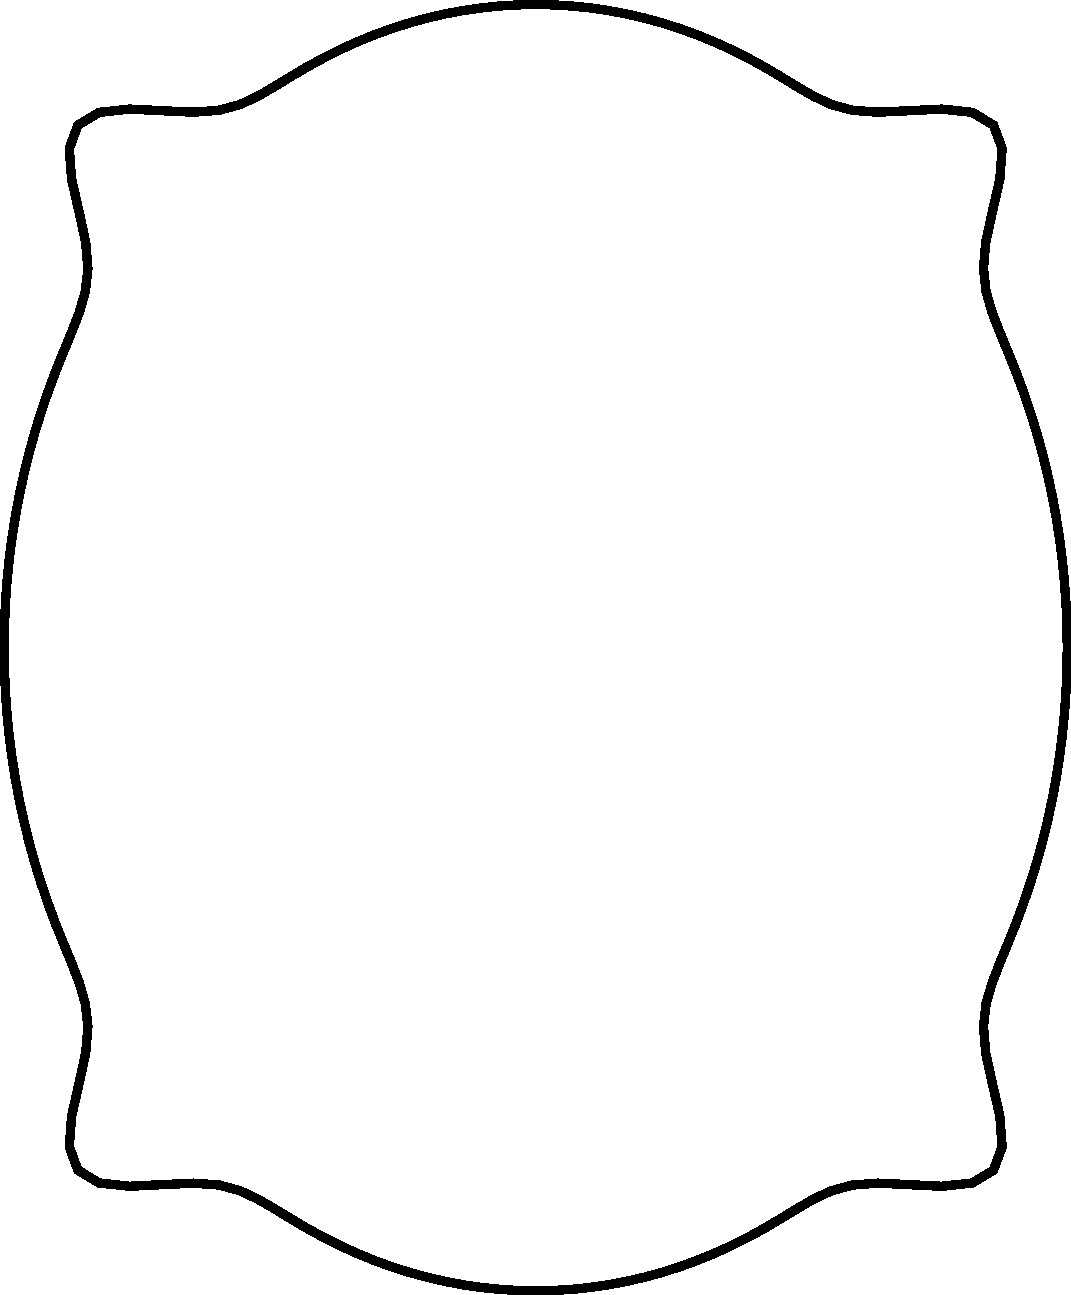
\includegraphics[width=.9\linewidth]{img/synthetic-generation/shapes/2.pdf}
	\end{subfigure}
	\begin{subfigure}[b]{0.24\textwidth}
		\centering
		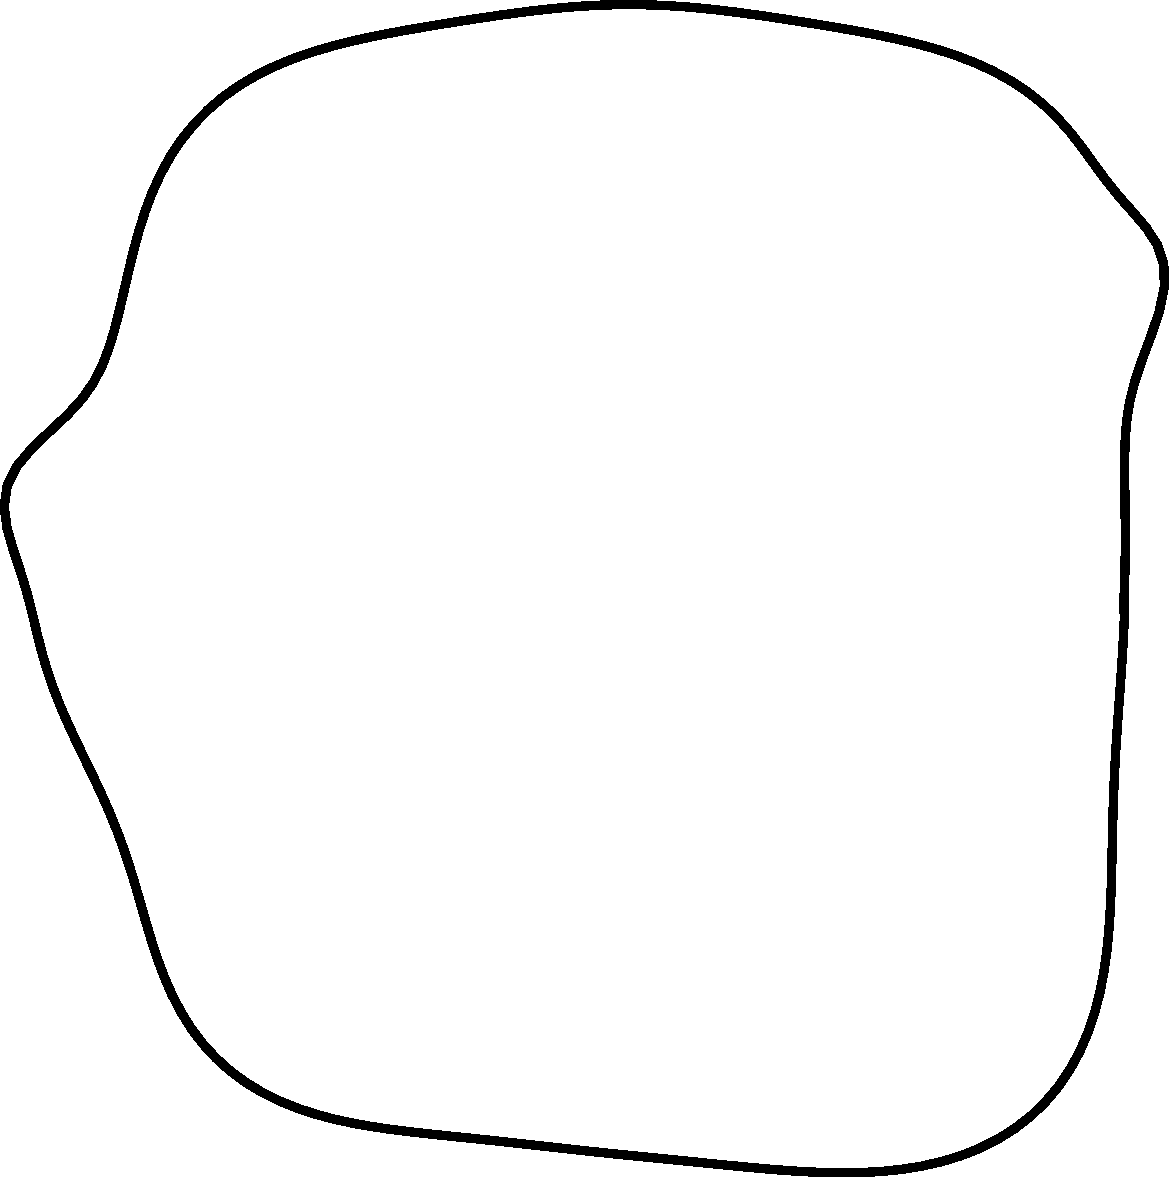
\includegraphics[width=.9\linewidth]{img/synthetic-generation/shapes/3.pdf}
	\end{subfigure}
	\begin{subfigure}[b]{0.24\textwidth}
		\centering
		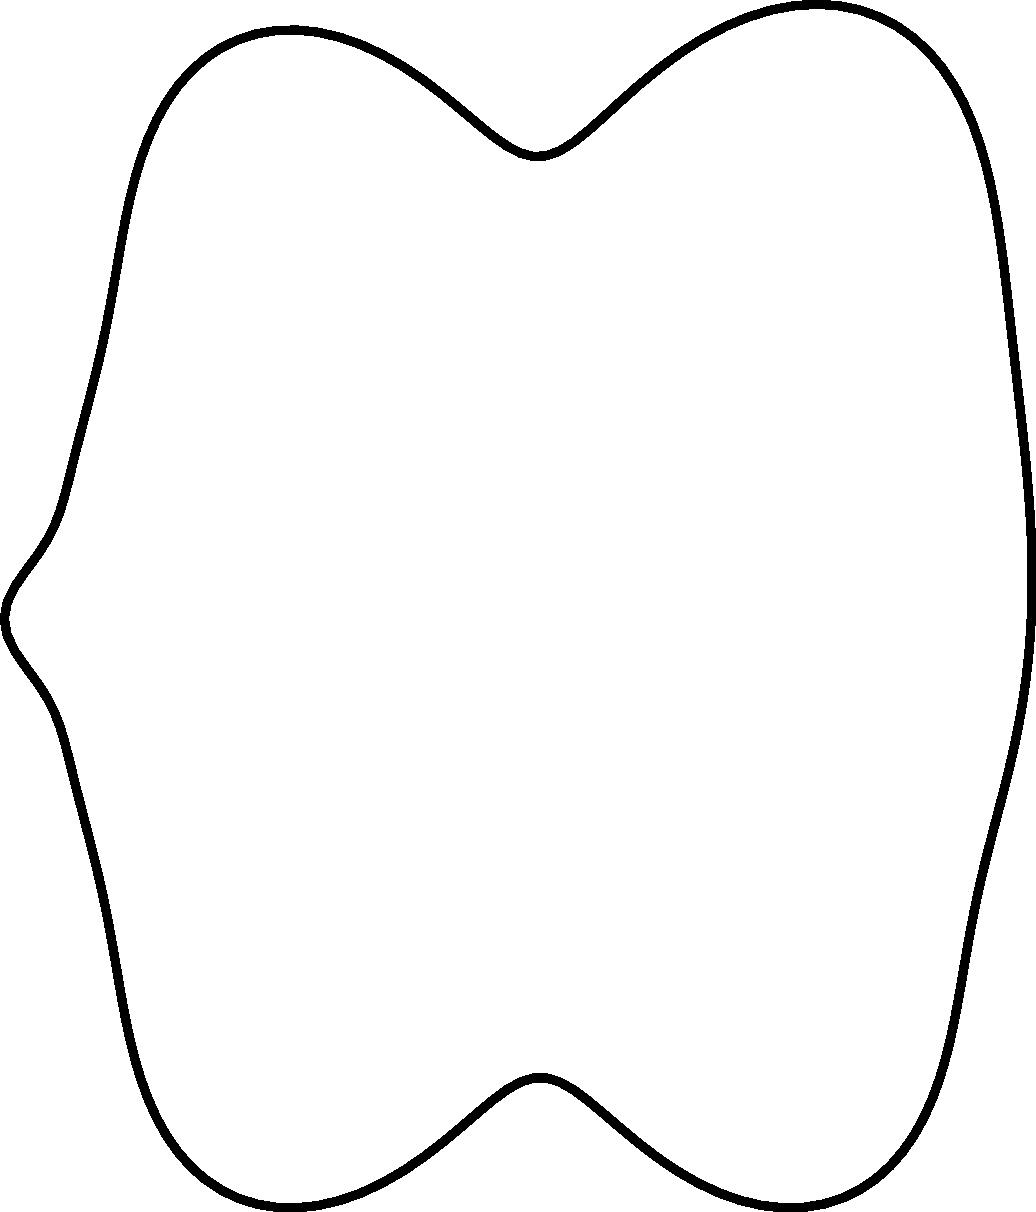
\includegraphics[width=.9\linewidth]{img/synthetic-generation/shapes/4.pdf}
	\end{subfigure}
	\caption{Shapes generated using synthetic generation}
	\label{fig:synthetic-shapes}
\end{figure}

The first step to testing with synthetic data is to define how the data should look like and how it is possible to generate such data. Since the algorithm compares two classes of data we need to create two sets of outlines that have similar characteristics, but also vary inside each set. Additionally because of the style of our algorithm we decided to create circle-shaped test-data. As the base for our data, we use a ellipsoid, which we can vary in eccentricity. Parameterized by angle the ellipsoid can be defined as, where $\epsilon$ is a parameter that defines the eccentricity of the ellipsoid:

\begin{equation}
\vec{e}(\alpha) = \left( \begin{array}{c}
cos(\alpha) \\
\epsilon sin(\alpha)
\end{array} \right) 
\end{equation}

To represent shape variations on the bone, we decided to use Gaussian bell curves, which can be stacked onto each other to produce a whole variation of shapes. Each of these bell curves $b_i(\alpha)$ is defined by a height $h_i$, an angle at which the curve has its center $\mu_i$ and a width of the curve $\sigma$. The formula for the curve is applied in the normal direction of the current angle $\vec{n}(\alpha)$, which is defined as:

\begin{equation}
\vec{n}(\alpha) = \frac{1}{\sqrt{(v_y^\prime(\alpha))^2 + (-v_x^\prime(\alpha))^2}}\left( \begin{array}{c}
v_y^\prime(\alpha) \\
-v_x^\prime(\alpha)
\end{array} \right)
\end{equation}

Using this normal vector the set of bell curves $B$ can be applied to the ellipsoid:

\begin{equation}
\vec{b}(\alpha) = \sum_{(h_i, \mu_i, \sigma_i) \in B}h_i \vec{n}(\alpha) \exp\left(\frac{-(\mu_i - \alpha)^2}{2 \sigma_i^2} \right )
\end{equation}

The whole shape can be defined by summing these functions together:

\begin{equation}
\vec{b}(\alpha) = \vec{e}(\alpha) + \vec{b}(\alpha)
\end{equation}

This function needs to be evaluated at $n$ angles $\alpha_i$ with $i = 1 ... n$ to get an outline that can be used as input for the algorithm.

\begin{equation}
\alpha_i = \frac{i}{n} 360^{\circ}
\end{equation}

This is the base for generating multiple shapes of this kind to feed the algorithm. Figure \ref{fig:synthetic-shapes} shows shapes that can be built using this method. Using these equations, we could only define two shapes using the described method. To describe two classes, we needed to add randomized elements to the equations.

The first randomized elements are class internal randomizations that describe differences in measurement and registration. For each class we can define standard deviations for radius $\sigma_r$, evaluation angles $\sigma_\alpha$ and transformation $\sigma_t$. Randomized values $n_r()$, $n_\alpha()$, $n_t$ based on normal distributions using these parameters are added whenever a value is accessed. The values are adapted as follows:

\begin{equation}
\begin{split}
& \vec{t} = \left( \begin{array}{c}
n_t() \\
n_t()
\end{array} \right) \\
& \vec{e}_r = \begin{pmatrix}
1 + n_r() & 0 \\
0 & 1 + n_r() \\
\end{pmatrix} \vec{e}  + \vec{t} \\
& \alpha_{ri} = \alpha_i + n_\alpha() \\
\end{split}
\end{equation}

Additionally the number of evaluation angles $n$ is chosen from a uniform distribution between $n_{min}$ and $n_{max}$.

Similarly to randomizing the overall shapes, the shape variations need to be randomized as well, since the features might occur at slightly different positions in nature. To do this we can add randomized elements to each of the parameters that define a shape variation.

\begin{equation}
\begin{split}
& h_{ir} = h_i + n_{hi}() \\
& \mu_{ir} = \mu_i + n_{\mu i}() \\
& \sigma_{ir} = \sigma_i + n_{\sigma i}() \\
\end{split}
\end{equation}

Using this randomization process two classes of semi-randomized data can be built that we can compare using the algorithm presented in Section \ref{sec:shape-comparison}. The classes are already registered, so the comparison is possible without further preprocessing. Since we define the characteristic locations on the bone outline ourselves, we can validate whether they are detected by the algorithm correctly.

\begin{figure}[h]
	\centering
	\begin{subfigure}[b]{0.24\textwidth}
		\centering
		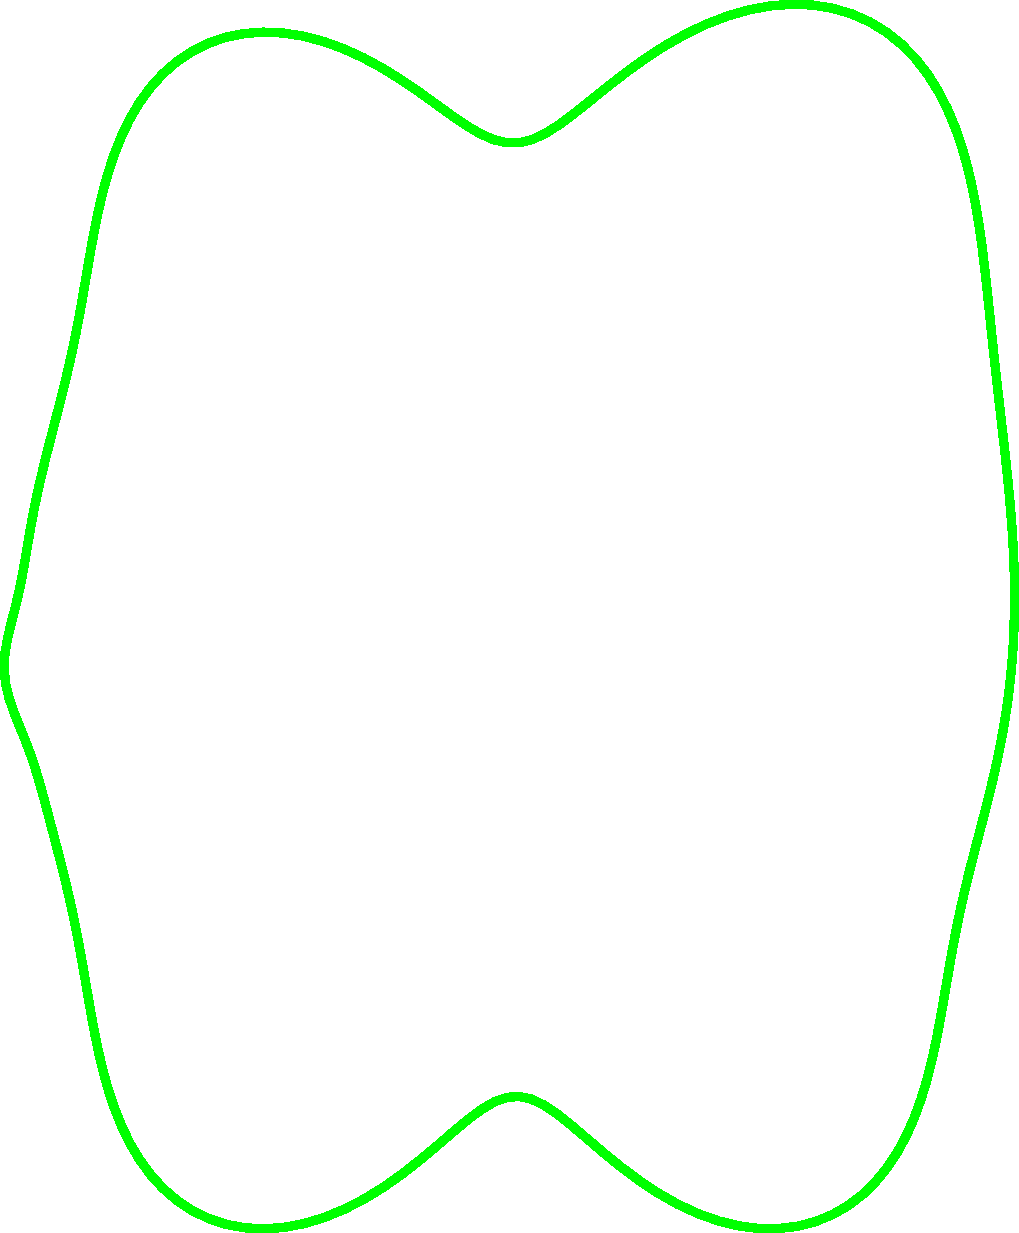
\includegraphics[width=.9\linewidth]{img/synthetic-generation/classes/1-1.pdf}
		\caption{Class A}
		\label{subfig:synthetic-classes:a-1}
	\end{subfigure}
	\begin{subfigure}[b]{0.24\textwidth}
		\centering
		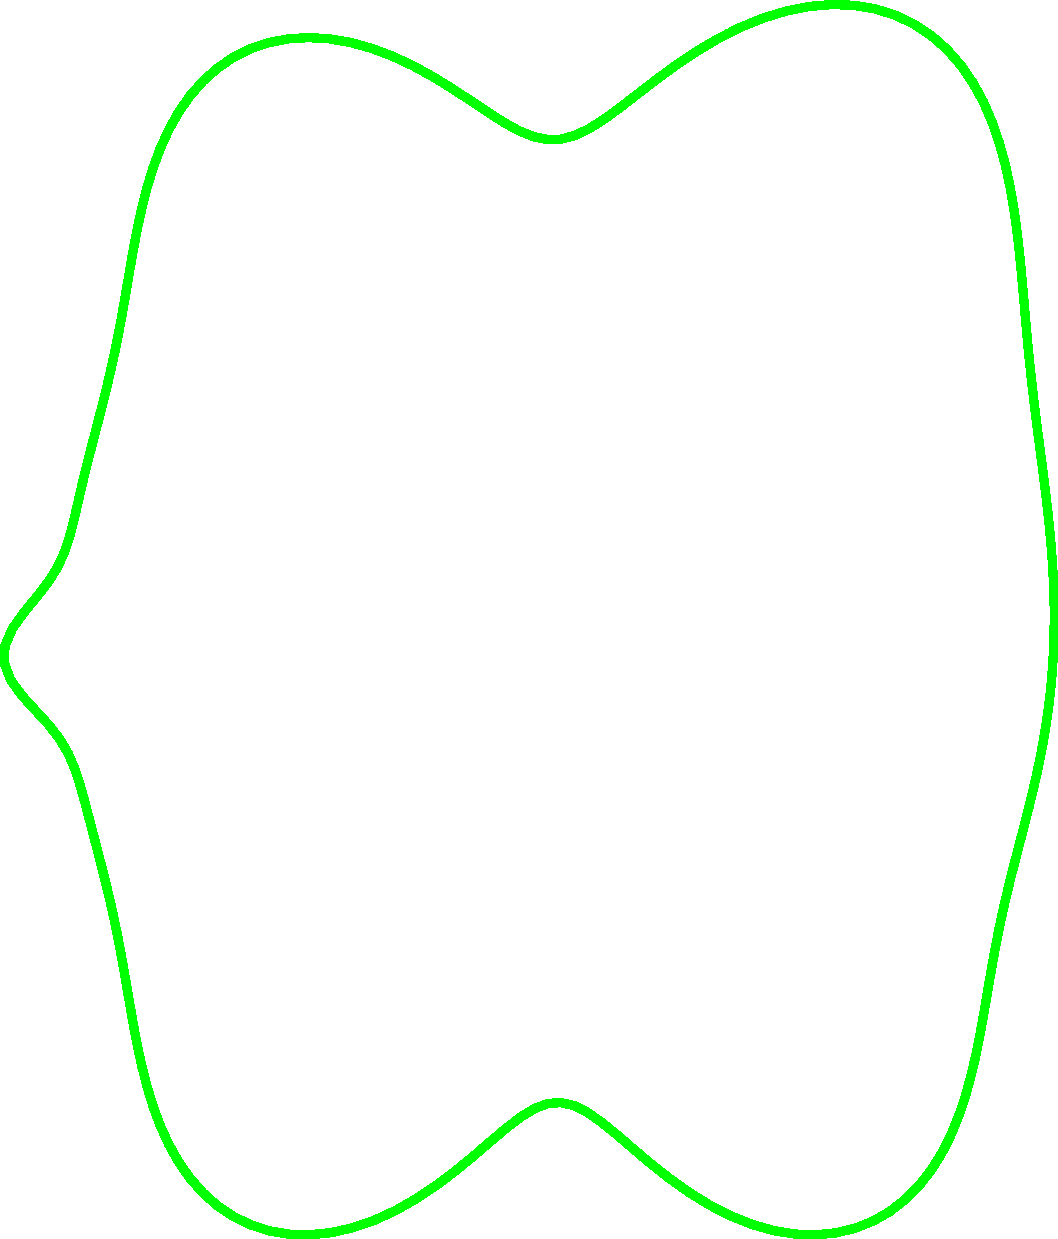
\includegraphics[width=.9\linewidth]{img/synthetic-generation/classes/1-2.pdf}
		\caption{Class A}
		\label{subfig:synthetic-classes:a-2}
	\end{subfigure}
	\begin{subfigure}[b]{0.24\textwidth}
		\centering
		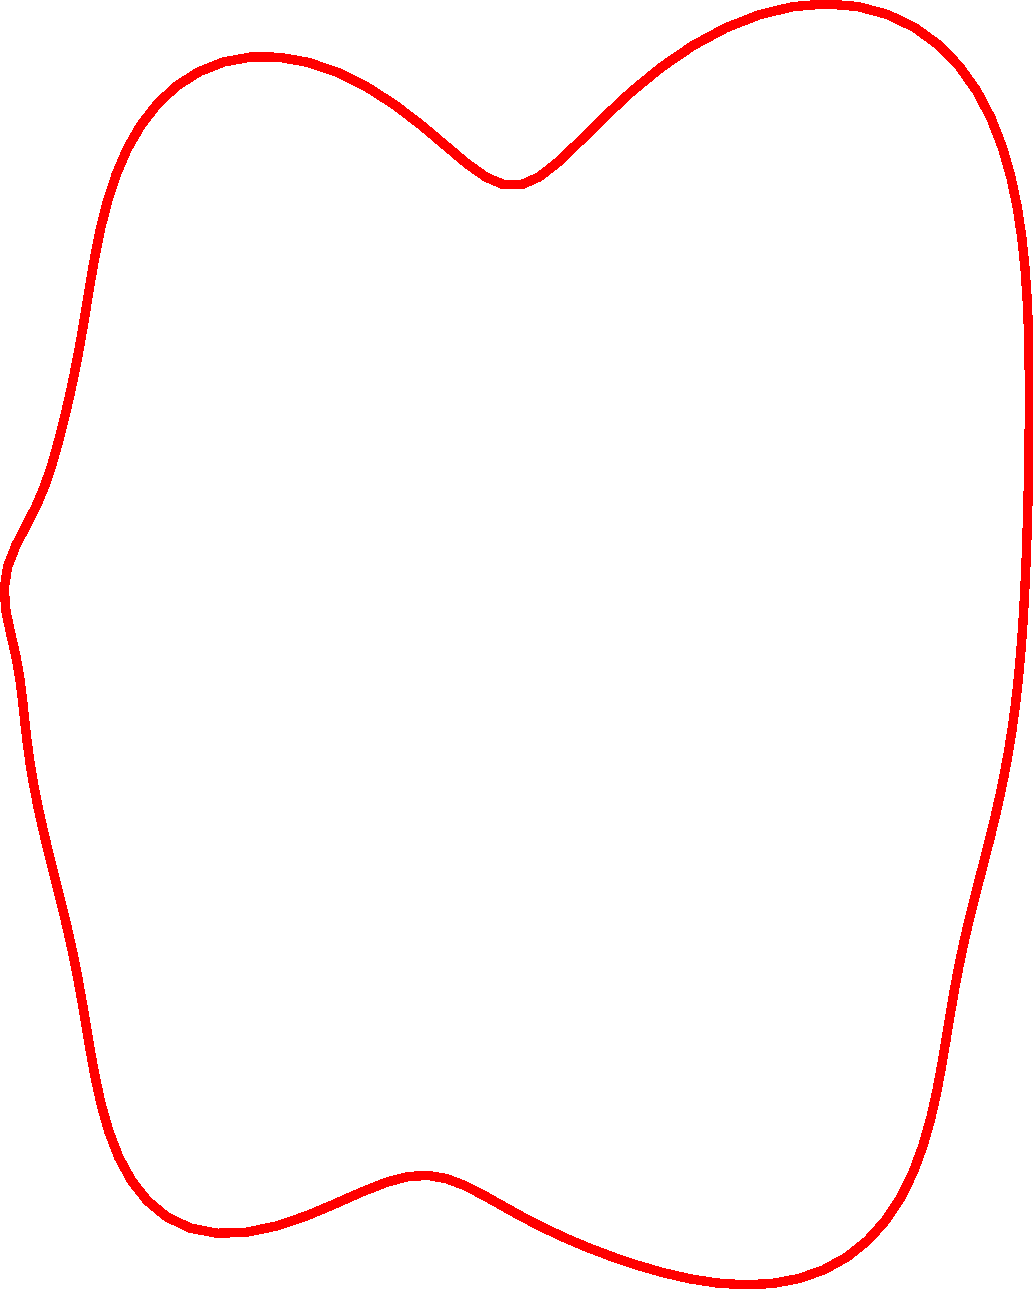
\includegraphics[width=.9\linewidth]{img/synthetic-generation/classes/2-1.pdf}
		\caption{Class B}
		\label{subfig:synthetic-classes:b-1}
	\end{subfigure}
	\begin{subfigure}[b]{0.24\textwidth}
		\centering
		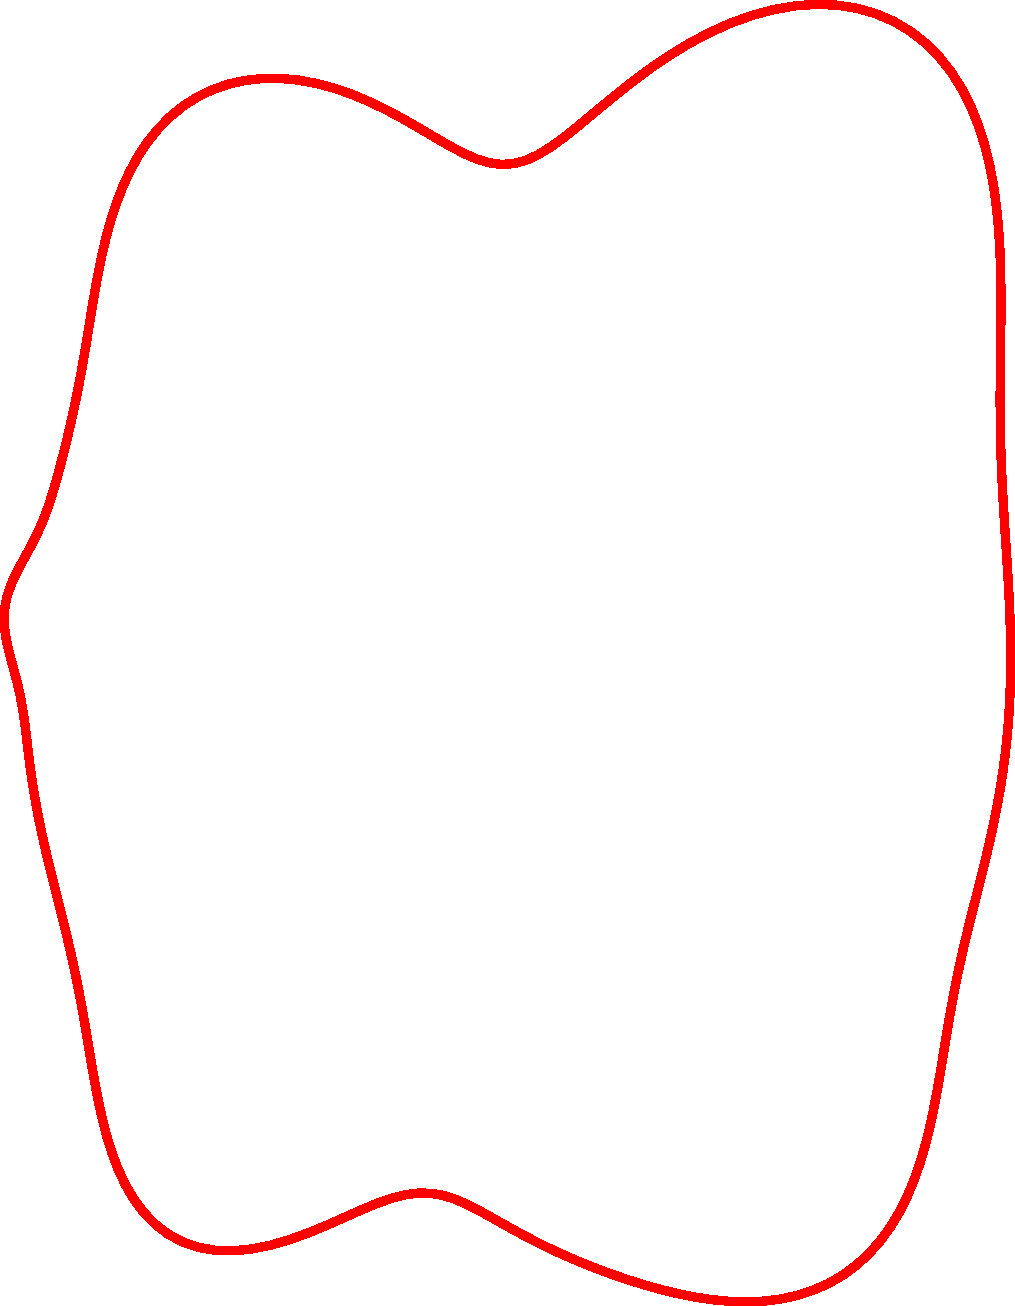
\includegraphics[width=.9\linewidth]{img/synthetic-generation/classes/2-2.pdf}
		\caption{Class B}
		\label{subfig:synthetic-classes:b-2}
	\end{subfigure}
	\caption{Two observations each for two classes of outlines that were synthetically generated}
	\label{fig:synthetic-classes}
\end{figure}

Figure \ref{fig:synthetic-classes} shows two classes that were generated using this process. The classes in this figure have their distinct variations in the position of the small left bulge, the location of the indentation at the bottom and the height of the right bulge at the top. It is also noticeable that the small left bulge is different inside of class A, because it is much more distinct in Figure \ref{subfig:synthetic-classes:a-2} than it is in Figure \ref{subfig:synthetic-classes:a-1}. The small left bulge is less distinct in Figure \ref{subfig:synthetic-classes:b-1} than it is in Figure \ref{subfig:synthetic-classes:b-2} as well. Additionally the indentation at the top more shallow in Figure \ref{subfig:synthetic-classes:b-2} than in \ref{subfig:synthetic-classes:b-1} and has slightly shifted to the right. 

Unless otherwise stated, we use 30 observation per class in our experiments. Randomization is only applied if it is explicitly tested, so it can not influence the results.

\subsection{Influence of Different Types of Variations in Shape Features}

The first test with randomized data has the goal of visualizing how certain changes in shape in between the classes materialize in the result. Since we cannot determine the type of shape shift from the separability metric itself, we need to know how these shape changes influence the separability metric and how we can determine them using the mean shapes of the classes in combination with the separability metric. For this purpose we determined several characteristic changes in shape that we tested using synthetic data based on the unit circle.

\subsubsection{Missing Characteristic}

A missing characteristic is a characteristic that appears in one class, but not in another.

\subsubsection{Less Distinct Characteristic}

\subsubsection{Shifted Characteristic}

\subsection{Influence of Variances in Shape Features}

\subsection{Influence of Errors in Shape Measurement}

\subsection{Influence of Errors in Shape Registration}

\chapter{Conclusion}

\section{Summary}

\section{Discussion}

\section{Future Work}

\appendix

\chapter{Landmark Extraction}

\begin{table}
    \begin{center}
        \begin{tabular}{|r|r|r|r|}
            \hline \makebox[3cm]{Landmark No} & \makebox[1cm]{$\alpha_{min}$} & \makebox[1cm]{$\alpha_{max}$} & \makebox[2cm]{Type} \\
            \hline\hline 1 &  $30^{\circ}$ & $90^{\circ}$ & maximum \\
            \hline 2 &  $80^{\circ}$ & $100^{\circ}$ & minimum \\
            \hline 3 &  $90^{\circ}$ & $150^{\circ}$ & maximum \\
            \hline 5 &  $170^{\circ}$ & $190^{\circ}$ & maximum \\
            \hline 6 &  $210^{\circ}$ & $270^{\circ}$ & maximum \\
            \hline 7 &  $260^{\circ}$ & $280^{\circ}$ & minimum \\
            \hline 8 &  $270^{\circ}$ & $330^{\circ}$ & maximum \\
            \hline
        \end{tabular}
    \end{center}
    \caption{Landmark Definitions for the Extraction by Angle.}
    \label{appendix:table:landmarks-angle}
\end{table}

\begin{table}
    \begin{center}
        \begin{tabular}{|r|r|r|r|r|r|r|}
            \hline
            \makebox[3cm]{Landmark No} & \makebox[1cm]{$x_{min}$} & \makebox[1cm]{$x_{max}$} & \makebox[1cm]{$y_{min}$} & \makebox[1cm]{$y_{max}$} & \makebox[2cm]{Axis} & \makebox[2cm]{Type} \\
            \hline
            \hline 1 &  $0.25$ & $1$ & $0.75$ & $1.5$ & y & maximum \\
            \hline 2 &  $-0.5$ & $0.5$ & $0.75$ & $1.5$ & y & minimum \\
            \hline 3 &  $-1$ & $-0.25$ & $0.75$ & $1.5$ & y & maximum \\
            \hline 5 &  $-1$ & $-0.25$ & $-0.3$ & $0.3$ & x & minimum \\
            \hline 6 &  $-1$ & $0.25$ & $-1.5$ & $-0.75$ & y & minimum \\
            \hline 7 &  $-0.5$ & $0.5$ & $-1.5$ & $-0.75$ & y & maximum \\
            \hline 8 &  $0.25$ & $1$ & $-1.5$ & $-0.75$ & y & minimum \\
            \hline
        \end{tabular}
    \end{center}
    \caption{Landmark Definitions for the Extraction by Space Partitioning.}
    \label{appendix:table:landmarks-space}
\end{table}

% Abbildungsverzeichnis (kann auch nach dem Inhaltsverzeichnis kommen)
\listoffigures

% Tabellenverzeichnis (kann auch nach dem Inhaltsverzeichnis kommen)
\listoftables

% Literaturverzeichnis
\bibliographystyle{dbstmpl}    % verwendet dbstmpl.bst
% alternative, vorinstallierte Stile sind z.B. plain oder abbrv
\bibliography{dbstmpl}         % verwendet dbstmpl.bib

\end{document}
